\documentclass[12pt,a4paper]{article}

% ======================
% Fonts (XeLaTeX only)
% ======================
\usepackage{fontspec}
% ======================
% Page layout
% ======================
\usepackage[
  a4paper,
  top=2.5cm,
  bottom=2.5cm,
  left=3cm,
  right=2.5cm,
  headheight=15pt
]{geometry}

\usepackage{enumitem}
% ======================
% Line breaking
% ======================
\usepackage{microtype}      % better justification, reduces hbox warnings
\usepackage{xurl}           % allows URLs to break anywhere
\sloppy                     % relaxes line-breaking strictness globally

\setmainfont{TeX Gyre Termes}   % Times-like academic font
\setsansfont{TeX Gyre Heros}

% Japanese font (important!)
\newfontfamily\japanesefont{Noto Serif CJK JP}

% ======================
% Languages
% ======================
\usepackage{polyglossia}

\setdefaultlanguage{spanish}
\setotherlanguage{english}

% ======================
% Bibliography
% ======================
\usepackage[
  backend=biber,
  style=ieee,
  sorting=nyt
]{biblatex}

\addbibresource{bibliography.bib}

\usepackage{mahjong}
\usepackage{tikz}
% ======================
% Tables & Figures
% ======================
\usepackage{graphicx}       % \includegraphics
\usepackage{float}          % [H] float placement
\usepackage{booktabs}       % \toprule, \midrule, \bottomrule
\usepackage{caption}        % better captions
\usepackage{subcaption}     % subfigures

% ======================
% Misc
% ======================
\usepackage{hyperref}       % clickable links/refs
\usepackage{xcolor}         % colors
\usepackage{microtype}      % better justification


\title{
Construcción de una IA de Mahjong mediante Transformers
}

\author{
Julia Ruiperez de Brito
}

\date{\today}

\begin{document}

\begin{titlepage}

\begin{center}

\vspace*{0.5cm}


\includegraphics[width=0.6\textwidth]{figures/usal_logo.png}


\vspace{0.5cm}

{\large Facultad de Ciencias}

\vspace{0.3cm}

{\large Grado en Ingeniería Informática}

\vspace{1cm}

{\Large \textbf{TRABAJO FIN DE GRADO}}

\vspace{0.8cm}

{\Huge \textbf{Desarrollo de una IA para jugar Riichi Mahjong}}

\vspace{0.25cm}

{\large \textit{Development of an AI to Play Riichi Mahjong}}

\vspace{0.8cm}

{\Large \textbf{Predicción y evaluación estratégica de descartes de Riichi Mahjong mediante Transformers}}

\vspace{0.25cm}

{\large \textit{Prediction and Strategic Evaluation of Riichi Mahjong Discards Using Transformers}}

\vspace{0.6cm}

\vfill

\begin{flushleft}

\textbf{Autor}\\
Julia Ruiperez de Brito

\vspace{0.5cm}

\textbf{Tutor}\\
Prof. Vidal Moreno Rodilla

\vspace{0.5cm}

\textbf{Departamento}\\
Informática y Automática

\end{flushleft}

\vfill

Salamanca\\
Septiembre 2026

\end{center}

\end{titlepage}


\clearpage

\input{frontmatter/acknowledgements}

\clearpage

\section*{Abstract}

This project presents an Artificial Intelligence system capable of selecting discard actions in Riichi Mahjong, a traditional Japanese game of imperfect information.

Using a Transformer-based architecture, the model is trained through imitation learning on a dataset composed of real games collected from Tenhou.net. The model is evaluated in terms of predictive accuracy, and the implications of the obtained results are discussed.

In addition to conventional accuracy metrics, this work proposes a complementary evaluation method referred to as \textit{Strategic Accuracy}. It uses categories defined through Shanten and Ukeire to analyse hand efficiency beyond exact agreement with the observed action.

On a reserved evaluation set containing 52,563 game states, the model trained on 500,000 states achieves a top-1 accuracy of 65.64\%, a top-3 accuracy of 92.47\%, and a strategic accuracy of 94.01\%. Compared with the checkpoint identified as 100k, the second model improves all predictive metrics and reduces Shanten-degrading decisions from 5.03\% to 1.59\%. These results indicate that the model learns relevant discard-selection patterns, although the proposed strategic evaluation remains limited to the aspects represented by Shanten and Ukeire.

\vspace{0.5cm}

\textbf{Keywords:}

Riichi Mahjong,
Artificial Intelligence,
Transformers,
Imitation Learning,
Strategic Accuracy,
Model Evaluation,
Imperfect Information Games.


\clearpage

\section*{Resumen}

Este trabajo presenta un sistema de Inteligencia Artificial capaz de tomar decisiones de descarte en Riichi Mahjong, un juego tradicional japonés de información imperfecta caracterizado por un elevado nivel de complejidad estratégica.

Para ello, se desarrolla un modelo basado en la arquitectura Transformer entrenado mediante aprendizaje por imitación a partir de un conjunto de datos compuesto por partidas reales obtenidas de la plataforma Tenhou.net. El rendimiento del modelo se evalúa utilizando métricas convencionales de precisión, analizando además las implicaciones de los resultados obtenidos.

Con el objetivo de complementar estas métricas tradicionales, se propone en este trabajo una metodología de evaluación denominada \textit{Precisión Estratégica}, basada en categorías definidas mediante Shanten y Ukeire. Este enfoque permite analizar la eficiencia de las decisiones generadas por el modelo más allá de la coincidencia exacta con la acción observada.

Los resultados experimentales muestran que el modelo entrenado con 500.000 estados alcanza una precisión exacta del 65,64\%, una precisión top-3 del 92,47\% y una precisión estratégica del 94,01\% sobre un conjunto reservado de 52.563 estados. En comparación con el checkpoint identificado como 100k, el segundo modelo mejora todas las métricas predictivas y reduce las decisiones que empeoran el Shanten del 5,03\% al 1,59\%. Estos resultados indican que el modelo aprende regularidades relevantes para la selección de descartes, aunque la evaluación estratégica queda limitada a los aspectos representados mediante Shanten y Ukeire.

\vspace{0.5cm}

\textbf{Palabras clave:}

Riichi Mahjong,
Inteligencia Artificial,
Transformers,
Aprendizaje por Imitación,
Precisión Estratégica,
Evaluación de Modelos,
Juegos de Información Imperfecta.


\clearpage

\tableofcontents

\clearpage

\listoffigures

\clearpage

\listoftables

\clearpage

\section{Introducción}

Riichi Mahjong es un juego de información imperfecta,
caracterizado por una elevada complejidad estratégica y por la presencia de
información oculta. Su espacio de estados se estima en el orden de $10^{48}$\cite{li2020suphx}.
Además, el orden de juego puede alterarse, ya que ciertas acciones, como el
\textit{pon}, el \textit{chi} o el \textit{kan}, permiten interrumpir la secuencia habitual de turnos. Esto incrementa aún más la complejidad del juego.

Este proyecto desarrolla una Inteligencia Artificial que predice una acción de descarte a partir de la información observable de un estado de juego,
que incluye información secuencial y estática. El modelo se basa en la arquitectura Transformer
y se entrena mediante aprendizaje por imitación utilizando 500.000 estados de juego reales
obtenidos de partidas de la plataforma Tenhou.net.

Durante el desarrollo del proyecto se obtienen diferentes métricas de precisión,
analizando tanto la coincidencia con el descarte observado como la precisión estratégica, que se basa en categorías semánticas propias del juego
calculadas mediante el \textit{Shanten} y el \textit{Ukeire}.

El esquema general de esta memoria comienza con
los objetivos del proyecto,
seguido de una sección de teoría, donde se explican
el juego de Mahjong y las heurísticas del juego,
así como la arquitectura de Transformers y el aprendizaje
por imitación.
Después, se realiza un repaso del estado del arte,
donde se analizan los trabajos relacionados con el juego de Mahjong y con el uso de Transformers en juegos de información imperfecta.
A continuación, se describen las herramientas utilizadas para el desarrollo del proyecto
y se explica su proceso de desarrollo, desde la preparación de los datos hasta el
entrenamiento del modelo y la evaluación de los resultados.
Finalmente, se presentan los resultados obtenidos y se discuten las conclusiones del proyecto.

El trabajo surgió inicialmente como un proyecto personal orientado a crear una IA de Mahjong que sirviese como apoyo para aprender a jugar mejor. A partir de esta idea inicial, el proyecto evolucionó hacia un trabajo académico de carácter exploratorio. Al comienzo no existía una arquitectura final ni un conjunto de herramientas previamente definido, por lo que las decisiones se tomaron de forma progresiva a partir de las pruebas realizadas y de los resultados obtenidos.

No se siguió una metodología formal concreta ni se estableció un calendario cerrado de hitos. El desarrollo fue iterativo e incremental: se probaron diferentes formas de representar los estados de juego, incluyendo una aproximación inicial mediante redes convolucionales, antes de adoptar una representación basada en tokens y una arquitectura Transformer. Esta solución resultó más natural para codificar los distintos elementos de un estado de Mahjong. De manera similar, la evaluación estratégica basada en Shanten y Ukeire no formaba parte del planteamiento inicial, sino que surgió durante el desarrollo al observar las limitaciones de la precisión exacta. Los cuadernos de Jupyter documentan estas iteraciones y permiten seguir la evolución del proyecto desde las primeras pruebas hasta los resultados finales.


\section{Objetivos}

El objetivo principal de este trabajo es conseguir desarrollar
una IA de Mahjong mediante la tecnología moderna de Transformers,
en contraste con los enfoques de otras IAs como Suphx\cite{li2020suphx} basado en 
Redes Convolucionales. Presentando los beneficios y limitaciones de 
el uso de los Transformers para juegos de información imperfecta.

Para conseguir estos objetivos, nos planteamos los siguientes hitos:



\section{Conceptos Teóricos}

\subsection{Reglas Básicas}

En un juego de Riichi Mahjong, contamos con 4 jugadores
de los cuales 1 es el \textit{Dealer}, representado por el viento \textbf{Este}.
Cada jugador recibe 13 piezas, que pueden ser de las siguientes:


\begin{table}[H]
\centering

\begin{tabular}{ll}

\toprule

\textbf{Suit} & \textbf{Tiles} \\

\midrule

Manzu (Caracteres)
&
\mahjong{123456789m}
\\[0.5em]

Pinzu (Circulos)
&
\mahjong{123456789p}
\\[0.5em]

Souzu (Bambús)
&
\mahjong{123456789s}
\\[0.5em]

Honores (Vientos y Dragones)
&
\mahjong{1234567z}
\\

\bottomrule

\end{tabular}

\caption{
Categorias de piezas de Riichi Mahjong
}

\label{tab:mahjong_tiles}

\end{table}

Las piezas de caracteres, circulos y bambús se numeran del 1 al 9, y las piezas de honores son, respectivamente, \textbf{Este}, \textbf{Sur}, \textbf{Oeste} y \textbf{Norte} para los vientos; y \textbf{Dragon Rojo}, \textbf{Dragon Verde} y \textbf{Dragon Blanco}. Cada una de estas piezas tienen 4 copias, por lo que en total son 136 piezas.

Inicialmente se decide si el juego durará una ronda de mesa \textbf{Este} o una ronda hasta \textbf{Sur}, donde la mesa obtiene ese viento, y aleatoriamente se escoge una persona para ser el \textit{Dealer}, que estará representado por la pieza del \textbf{Este} y se sentará en esa posición. Cada posición de jugadores está en un viento, como podemos ver en la siguiente imágen:

\begin{figure}[H]
\centering

\begin{tikzpicture}[scale=1.5]

% Mesa
\draw[thick] (-2,-2) rectangle (2,2);

% Centro
\node at (0,0) {\Large Mesa};

% Vientos
\node at (0,2.8) {\mahjong{4z}};
\node at (0,2.4) {Norte};

\node at (2.8,0) {\mahjong{1z}};
\node at (2.8,-0.4) {Este};

\node at (0,-2.6) {\mahjong{2z}};
\node at (0,-3.0) {Sur};

\node at (-2.8,0) {\mahjong{3z}};
\node at (-2.8,-0.4) {Oeste};

% Jugadores
\node at (0,-3.5) {Jugador 1};
\node at (3.8,0) {Jugador 0};
\node at (0,3.4) {Jugador 3};
\node at (-3.8,0) {Jugador 2};

\end{tikzpicture}

\caption{
Posición relativa de los jugadores y vientos en una mesa de Riichi Mahjong.
}

\label{fig:winds_table}

\end{figure}

El objetivo del juego es ganar las manos mediante \textit{Yaku} (combinaciones de manos que pueden ganar), de forma similar al poker. Se puede ver en el Anexo 1 una lista de \textit{Yaku} oficiales.


Cada jugador recibe 13 piezas, y su turno se basa de forma sencilla, a comprar una pieza y descartar otra, hasta que la mano se complete (si posible). 
Al momento de completar una mano preparada para ganar, esto es, que falta solo una pieza para ganar (\textit{Tenpai}), el jugador puede ganar cogiendo la pieza de la compra normal, o del descarte de otro jugador. De este modo, los jugadores también deben evitar descartar la pieza que completa la mano de otro jugador, ya que pierde puntos de este modo. En resumen, las formas de ganar son las siguientes:

\begin{table}[H]
\centering
\begin{tabular}{|l|l|}
\hline
\textbf{Forma de Ganar} & \textbf{Descripción} \\
\hline
\textbf{Tsumo} & Ganar con la pieza de la compra normal. \\
\textbf{Ron} & Ganar con la pieza del descarte de otro jugador. \\
\hline
\end{tabular}
\caption{
Formas de ganar en Riichi Mahjong
}
\label{tab:winning-conditions}
\end{table}

El juego también dispone de una pared de piezas, donde se encuentra la llamada \textbf{Pared Muerta} (\textit{Dead Wall}) que contiene 14 piezas que nunca se verán dentro del juego, estas 14 piezas son escogidas aleaatóriamente al inicio de cada ronda. Además, esta pared muerta contiene lo que llamamos indicadores de \textit{dora}, que son piezas que adicionan puntos a la mano ganadora. El número del indicador revela que la próxima pieza es el \textit{dora}, y por lo tanto vale más puntos. Para los vientos, el orden de dora es Este $\rightarrow$ Sur $\rightarrow$ Oeste $\rightarrow$ Norte $\rightarrow$ Este, y para los dragones es Rojo $\rightarrow$ Verde $\rightarrow$ Blanco $\rightarrow$ Rojo. Para las piezas de caracteres, circulos y bambús, el orden es 1 $\rightarrow$ 2 $\rightarrow$ 3 $\rightarrow$ ... $\rightarrow$ 9 $\rightarrow$ 1.

Durante el juego, un jugador tiene la opción de hacer "llamadas", estas llamadas se resumen a coger el descarte de otro jugador para completar un trio o una secuencia, también se puede utilizar para completar una cuadrupla, que abrirá otro indicador dora, pudiendo aumentar el valor de tu mano o de una mano rival. Sin embargo, hacer llamadas también tiene la contra parte de que tu mano ya no es cerrada, y por lo tanto no podrás declarar \textit{Riichi} como veremos a continuación.

La regla más importante del Riichi Mahjong: hacer \textbf{\textit{Riichi}}: Cuando un jugador está en \textit{Tenpai} y tiene la mano cerrada, tiene la opción de declarar \textit{Riichi}, que nada más es una apuesta de 1000 puntos a que ganará la mano. Esto bloquea la  mano del jugador y solo podrá comprar y descartar piezas sin poder modificar más su mano, siendo la única opción posible hacer \textit{Tsumo} o \textit{Ron}\ref{tab:winning-conditions}.

Por lo tanto, podemos ver en la siguiente tabla un resumen de las acciones posibles en cada turno:

\begin{table}[H]
\centering
\begin{tabular}{|l|p{0.6\textwidth}|}
\hline
\textbf{Acción} & \textbf{Descripción} \\
\hline
\hline
Comprar & Tomar una pieza de la pared. \\
\hline
Descartar & Descartar una pieza de la mano. \\
\hline
Declarar \textit{Riichi} & Apostar 1000 puntos a que ganará la mano. \\
\hline
\textit{Pon} & Coger el descarte de otro jugador para completar un trio. \\
\hline
\textit{Chi} & Coger el descarte de otro jugador para completar una secuencia. \\
\hline
\textit{Kan} & Completar una cuadrupla (puede ser de tu mano sin abrir). \\
\hline
\end{tabular}
\caption{
Acciones posibles en cada turno de Riichi Mahjong
}
\label{tab:actions}
\end{table}

Con esto finalizamos la explicación de las reglas básicas del juego, y a continuación se explicarán los conceptos de estrategia y teoría que se utilizan para jugar el juego de forma óptima.

\section{Estado Del Arte}

La Inteligencia Artificial capaz dde jugar al Majong más conocida e importante es Suphx\cite{li2020suphx}, una IA creada por Microsoft utilizando una arquitectura de CNNs (Redes Neuronales Convolucionales) que después pasa por una arquitectura de RL (Reinforcement Learning). Suphx obtuvo resultados de 

\section{Herramientas y Entorno de Desarrollo}

El desarrollo del proyecto se ha realizado principalmente utilizando el lenguaje de programación Python, empleando un entorno virtual gestionado mediante Conda y aceleración por GPU mediante CUDA para el entrenamiento de los modelos desarrollados con la biblioteca PyTorch.

El proceso de trabajo ha sido eminentemente iterativo y experimental, sin seguir una metodología formal concreta. En lugar de partir de un diseño definitivo, el proyecto avanzó mediante pruebas sucesivas documentadas en cuadernos de Jupyter Notebook. Estos cuadernos permiten registrar las principales etapas del desarrollo: exploración inicial del conjunto de datos, pruebas de diferentes representaciones del estado, construcción progresiva de la arquitectura Transformer, validación mediante pruebas de sobreajuste, entrenamiento a diferentes escalas y análisis estratégico de los resultados obtenidos.

Este enfoque ha facilitado la experimentación continua con distintos tamaños de conjunto de datos, configuraciones de entrenamiento y métricas de evaluación. Algunas decisiones importantes, como el uso de una representación mediante tokens o la incorporación de la evaluación estratégica, surgieron como resultado de estas iteraciones y no de una planificación cerrada desde el inicio.

Todo el código fuente del proyecto, así como los distintos experimentos realizados, se encuentran versionados mediante Git y alojados en un repositorio público de GitHub:

\begin{center}
\url{https://github.com/Ruipi/tfg}
\end{center}

Los experimentos de entrenamiento se ejecutaron sobre un equipo equipado con una GPU NVIDIA GeForce RTX 5060 Laptop, lo que permitió acelerar significativamente el proceso de entrenamiento del modelo Transformer y realizar múltiples iteraciones experimentales en tiempos razonables.

\begin{table}[H]
\centering

\begin{tabular}{ll}

\toprule
Elemento & Herramienta \\
\midrule

Lenguaje & Python 3.11 \\
Gestión de entorno & Conda (Miniforge) \\
Deep Learning & PyTorch \\
GPU & CUDA \\
Visualización & Matplotlib, Seaborn \\
Análisis de datos & Pandas, NumPy \\
Base de datos & SQLite \\
Desarrollo experimental & Jupyter Notebook \\
Control de versiones & Git + GitHub \\
Editor & Visual Studio Code \\

\bottomrule

\end{tabular}

\caption{Tecnologías empleadas durante el desarrollo del proyecto.}

\end{table}


\section{Desarrollo del Proyecto}

En esta sección explicaremos como ha sido desarrollado el proyecto, empezando por el Análisis de Exploración de Datos (EDA); el planteamiento de la arquitectura, donde se verán las decisiones tomadas para la construcción del modelo; la construcción del modelo; y las iteraciones de desarrollo.

\subsection{Análisis de Exploración de Datos}

El conjunto de datos utilizado procede de registros de partidas de Tenhou recopilados mediante la herramienta \textit{phoenix-logs} y transformados a una base de datos SQLite mediante \textit{tenhou\_dataprocess}. El dataset se distribuye a través de Kaggle con licencia Apache 2.0 y contiene ocho tablas asociadas a diferentes tipos de decisiones: \textit{Discard}, \textit{Riichi}, \textit{Chi}, \textit{Pon}, \textit{DaiMinKan}, \textit{ShouMinKan}, \textit{AnKan} y \textit{Skip}. Cada registro almacena un estado de juego serializado en formato JSON y comprimido mediante gzip.

En este proyecto se utiliza exclusivamente la tabla \textit{Discard}. A partir de ella se construyó una base de datos filtrada que conserva únicamente los estados con más de una alternativa de descarte, obteniéndose un total de 552.563 estados.

\begin{table}[H]
  \centering
  \caption{Schemas del Dataset}
  \label{tab:schemas}
  \begin{tabular}{@{}cll@{}}
    \toprule
    \textbf{ID} & \textbf{Nombre} & \textbf{Descripción} \\
    \midrule
    0 & Skip        & No realizar ninguna acción; pasar el turno. \\
    1 & Discard     & Descartar una ficha de la mano. \\
    2 & Chi         & Robar la ficha descartada por el jugador anterior para formar una secuencia. \\
    3 & Pon         & Robar la ficha descartada por cualquier jugador para formar un trío. \\
    4 & DaiMinKan   & Robar la ficha descartada por cualquier jugador para formar un cuádruple abierto. \\
    5 & ShouMinKan  & Añadir una ficha propia a un trío abierto (Pon) para formar un cuádruple. \\
    6 & AnKan       & Declarar un cuádruple cerrado con cuatro fichas de la propia mano. \\
    7 & Riichi      & Declarar \textit{Tenpai} con la mano cerrada, apostando 1000 puntos. \\
    \bottomrule
  \end{tabular}
\end{table}

Y a partir de ellos, se analizaron los siguientes datos.

\subsection{Distribución de Acciones}

\begin{figure}[H]
  \centering
  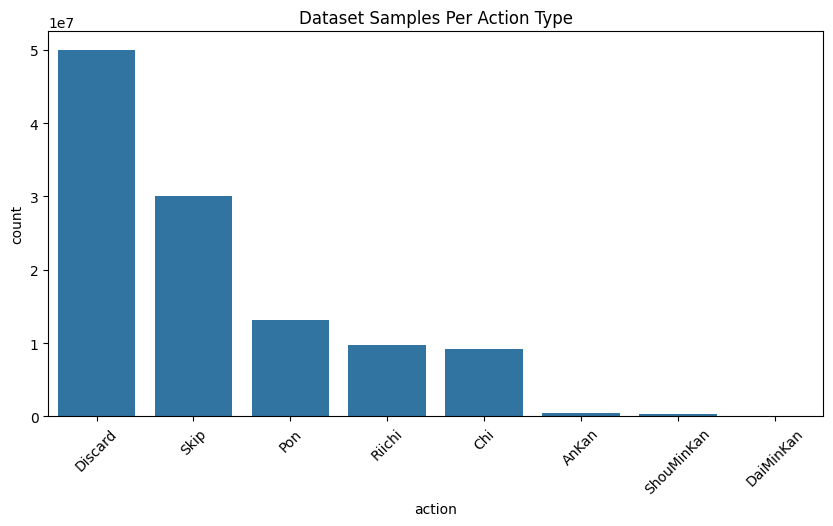
\includegraphics[width=0.8\textwidth]{figures/distribucion_acciones.png}
  \caption{Distribución de Número de Datos del Dataset por tipo de Acciones Válidas}
  \label{fig:dist_acciones_validas}
\end{figure}

En este gráfico se observa un fuerte desequilibrio entre los tipos de acciones. Los descartes son mucho más frecuentes que las llamadas o los distintos tipos de Kan, por lo que el presente trabajo se centra exclusivamente en los estados cuya acción observada es un descarte. El tratamiento conjunto de todas las decisiones requeriría considerar este desequilibrio y queda fuera del alcance del modelo desarrollado.

\subsection{Distribución de la Suma de Acciones Válidas de una Sample}

\begin{figure}[H]
  \centering
  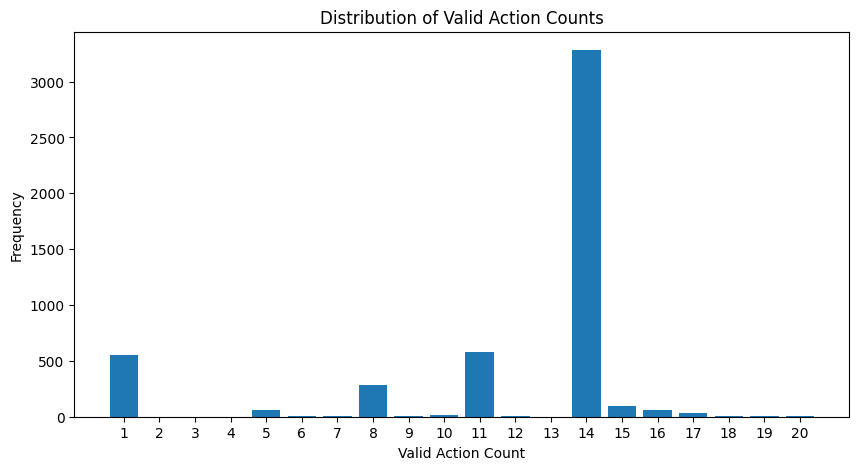
\includegraphics[width=0.8\textwidth]{figures/acciones_validas_dist.png}
  \caption{Distribución del número de acciones válidas del schema de Descarte}
  \label{fig:discard_valid_count}
\end{figure}

La mayor concentración ocurre en 14 acciones válidas, ya que una mano cerrada dispone normalmente de 14 fichas antes del descarte. También aparecen concentraciones en 11, 8 y 5 alternativas, asociadas a manos con una, dos o tres combinaciones abiertas, respectivamente, como se resume en la siguiente tabla:

\begin{table}[H]
  \centering
  \caption{Acciones válidas según melds abiertos}
  \label{tab:acciones_melds}
  \begin{tabular}{@{}cc@{}}
    \toprule
    \textbf{Acciones válidas} & \textbf{\textit{Melds} abiertos} \\
    \midrule
    11 & 1 \\
    8  & 2 \\
    5  & 3 \\
    2  & 4 \\
    \bottomrule
  \end{tabular}
\end{table}

Los estados con dos alternativas son menos frecuentes y suelen corresponder a manos con cuatro combinaciones ya formadas.

La base original contiene además numerosos estados con una única alternativa de descarte, situación habitual después de declarar \textit{Riichi}. Como en esos casos no existe una elección real entre varios descartes, se eliminaron para evitar que incrementasen artificialmente la precisión. La base filtrada conserva únicamente estados con más de una acción de tipo descarte.

Finalmente, el número de acciones válidas restante se explica debido a posibles acciones de \textit{Riichi} con diferentes piezas. 

\subsection{Frecuencia de Piezas Descartadas}

\begin{figure}[H]
  \centering
  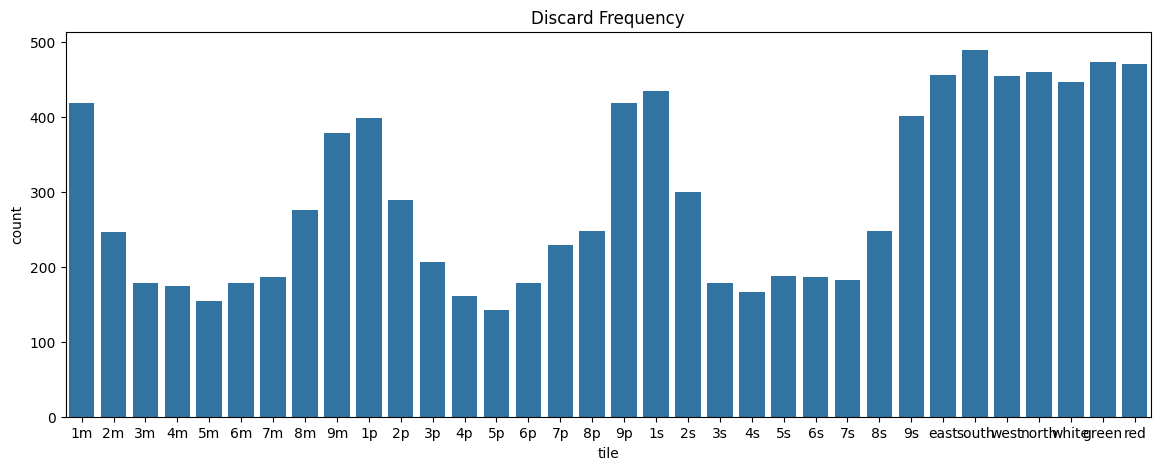
\includegraphics[width=0.8\textwidth]{figures/mostcommondiscarded.png}
  \caption{Frecuencia de las Piezas Descartadas}
  \label{fig:common_discarded}
\end{figure}

En este gráfico se observa que las fichas descartadas con mayor frecuencia son los honores (vientos y dragones), véase la Tabla \ref{tab:mahjong_tiles}, y las fichas terminales (unos y nueves). Una posible explicación es que, en muchas configuraciones de mano, estas fichas ofrecen menos posibilidades de formar secuencias que las fichas numeradas intermedias. Esta interpretación es descriptiva y no implica que deban descartarse siempre, ya que la decisión depende del estado concreto de la partida.

\subsection{Representación de un Estado}


Esta es la representación de un estado de mahjong dentro del Dataset:

\begin{lstlisting}[language=json, caption={Ejemplo de un estado}]
{
    {'round_wind': 0,
 'num_honba': 1,
 'num_riichi': 0,
 'player_wind': 0,
 'position': 0,
 'remain_tiles': 15,
 'dora_indicators': [7, 5],
 'hand_tiles': [1, 1, 2, 3, 3, 12, 13, 18, 19, 22, 22],
 'players': {'0': {'points': 41700,
   'riichi': False,
   'discards': [28, 27, 9, 16, 10, 6, 15, 20, 13, 32, 32, 0, 33, 33],
   'melds': [{'type': 2, 'tiles': [92, 98, 103, -1], 'who': [0, 0, 3, -1]}],
   'tsumo_giri': [0, 0, 0, 1, 0, 0, 1, 0, 0, 1, 1, 0, 0, 0]},
  '1': {'points': 19000,
   'riichi': False,
   'discards': [30, 27, 32, 18, 31, 17, 26, 26, 24, 2, 0, 14, 30, 10],
   'melds': [],
   'tsumo_giri': [0, 0, 0, 1, 0, 0, 0, 0, 1, 0, 1, 0, 0, 0]},
  '2': {'points': 20300,
   'riichi': False,
   'discards': [18, 17, 11, 16, 24, 25, 28, 23, 33, 32, 20, 7, 30, 17],
   'melds': [{'type': 5, 'tiles': [124, 126, 127, 125], 'who': [2, 2, 1, 2]},
    {'type': 2, 'tiles': [5, 13, 10, -1], 'who': [2, 2, 1, -1]}],
   'tsumo_giri': [0, 0, 0, 1, 0, 0, 0, 1, 0, 1, 1, 0, 1, 1]},
  '3': {'points': 19000,
   'riichi': False,
   'discards': [28, 29, 30, 18, 0, 11, 9, 27, 27, 0, 29, 26, 24, 25],
   'melds': [],
   'tsumo_giri': [0, 0, 0, 0, 0, 0, 1, 0, 0, 1, 1, 0, 0, 1]}},
 'valid_actions': [{'type': 1, 'tiles': [1], 'who': [0, -1, -1, -1]},
  {'type': 1, 'tiles': [1], 'who': [0, -1, -1, -1]},
  {'type': 1, 'tiles': [2], 'who': [0, -1, -1, -1]},
  {'type': 1, 'tiles': [3], 'who': [0, -1, -1, -1]},
  {'type': 1, 'tiles': [3], 'who': [0, -1, -1, -1]},
  {'type': 1, 'tiles': [12], 'who': [0, -1, -1, -1]},
  {'type': 1, 'tiles': [13], 'who': [0, -1, -1, -1]},
  {'type': 1, 'tiles': [18], 'who': [0, -1, -1, -1]},
  {'type': 1, 'tiles': [19], 'who': [0, -1, -1, -1]}],
 'action_idx': 7}
}
\end{lstlisting}

De este registro se obtiene la siguiente información:

\begin{table}[H]
  \centering
  \caption{Campos de un Estado de Mahjong}
  \label{tab:state_fields}
  \begin{tabular}{@{}clp{8cm}@{}}
    \toprule
    \textbf{Campo} & \textbf{Tipo} & \textbf{Descripción} \\
    \midrule
    round\_wind & int & Identificador de ronda utilizado por el dataset \\
    num\_honba & int & Número de honba \\
    num\_riichi & int & Número de riichi's (0-3) \\
    player\_wind & int & Viento del jugador (0-3) \\
    position & int & Posición del jugador (0-3) \\
    remain\_tiles & int & Número de fichas restantes en el muro (0-70) \\
    dora\_indicators & list[int] & Indicadores de dora en codificación Tenhou (0-135) \\
    hand\_tiles & list[int] & Fichas de la mano en codificación Tenhou (0-135) \\
    players & dict[int, dict] & Información de los jugadores, incluyendo puntos, riichi, descartes, melds y tsumo\_giri. \\
    valid\_actions & list[dict] & Lista de acciones válidas para el jugador actual. \\
    action\_idx & int & Índice de la acción tomada por el jugador actual. \\
    \bottomrule
  \end{tabular}
\end{table}

De estos datos, podemos aún extraer los campos de players:

\begin{table}[H]
  \centering
  \caption{Campos de un Jugador en un Estado de Mahjong}
  \label{tab:player_fields}
  \begin{tabular}{@{}clp{8cm}@{}}
    \toprule
    \textbf{Campo} & \textbf{Tipo} & \textbf{Descripción} \\
    \midrule
    points & int & Puntos del jugador (0-50000) \\
    riichi & bool & Indica si el jugador ha declarado riichi (True/False) \\
    discards & list[int] & Lista de fichas descartadas por el jugador (0-33) \\
    melds & list[dict] & Lista de combinaciones del jugador, cada una con tipo, fichas y procedencia. \\
    tsumo\_giri & list[int] & Lista indicando si cada ficha fue descartada inmediatamente después de ser robada (1) o no (0). \\
    \bottomrule
  \end{tabular}
\end{table}

Campos de melds:

\begin{table}[H]
  \centering
  \caption{Campos de un Meld en un Estado de Mahjong}
  \label{tab:meld_fields}
  \begin{tabular}{@{}clp{8cm}@{}}
    \toprule
    \textbf{Campo} & \textbf{Tipo} & \textbf{Descripción} \\
    \midrule
    type & int & Tipo de meld (2: Pon, 3: Chii, 4: DaiMinKan, 5: ShouMinKan, 6: AnKan) \\
    tiles & list[int] & Fichas que componen el meld en codificación Tenhou (0-135) \\
    who & list[int] & Lista indicando quién contribuyó a cada ficha del meld (-1 para fichas propias, 0-3 para otros jugadores) \\
    \bottomrule
  \end{tabular}
\end{table}

Y, por fin, campos de valid\_actions:

\begin{table}[H]
  \centering
  \caption{Campos de una Acción Válida en un Estado de Mahjong}
  \label{tab:valid_action_fields}
  \begin{tabular}{@{}clp{8cm}@{}}
    \toprule
    \textbf{Campo} & \textbf{Tipo} & \textbf{Descripción} \\
    \midrule
    type & int & Tipo de acción (0: Skip, 1: Discard, 2: Chi, 3: Pon, 4: DaiMinKan, 5: ShouMinKan, 6: AnKan, 7: Riichi, 8: Ron, 9: Tsumo, 10: Kyushukyuhai, 11: Chankan) \\
    tiles & list[int] & Fichas involucradas en la acción en codificación Tenhou (0-135) \\
    who & list[int] & Lista indicando quién realiza la acción y quién contribuye a ella (-1 para el jugador actual, 0-3 para otros jugadores) \\
    \bottomrule
  \end{tabular}
\end{table}


\section{Arquitectura del Modelo}
\label{sec:model-architecture}

Como se explicó en la Subsección \ref{subsec:transformer}, el modelo desarrollado en este trabajo utiliza una arquitectura basada en el codificador de un Transformer. La elección de una arquitectura de tipo \textit{encoder-only} se debe a que el objetivo del sistema no consiste en generar una secuencia de salida, sino en analizar la representación disponible de un estado de Riichi Mahjong y puntuar las acciones candidatas proporcionadas por el dataset.

La Figura \ref{fig:model-architecture} muestra el flujo general de procesamiento, desde la normalización de la instantánea almacenada en el conjunto de datos hasta la predicción final realizada por el modelo.

\begin{figure}[H]
    \centering

    \begin{tikzpicture}[
        node distance=0.55cm,
        font=\small,
        >=Latex,
        block/.style={
            rectangle,
            rounded corners=2mm,
            draw=black!65,
            line width=0.7pt,
            align=center,
            minimum height=1.05cm,
            text width=6.2cm,
            fill=black!3
        },
        process/.style={
            block,
            fill=blue!7
        },
        neural/.style={
            block,
            fill=orange!10
        },
        output/.style={
            block,
            fill=green!10
        },
        arrow/.style={
            ->,
            line width=0.8pt,
            draw=black!70
        },
        annotation/.style={
            font=\scriptsize,
            text=black!65,
            align=center
        }
    ]

    % Entrada y procesamiento
    \node[block] (raw) {
        \textbf{Datos de Tenhou}\\
        Estado almacenado en la base de datos
    };

    \node[process, below=of raw] (parser) {
        \textbf{Normalización del estado}\\
        Mano, descartes, melds, dora, vientos y contexto de la ronda
    };

    \node[process, below=of parser] (tokens) {
        \textbf{Tokenización}\\
        Conversión del estado canónico en una secuencia de identificadores
    };

    % Representación
    \node[neural, below=of tokens] (embedding) {
        \textbf{Capa de embeddings}\\
        Proyección de cada token a un vector continuo de dimensión $d_{\text{model}}$
    };

    \node[neural, below=of embedding] (encoder) {
        \textbf{Transformer Encoder}\\
        Self-attention multi-cabeza, red feed-forward, conexiones residuales
        y normalización
    };

    \node[neural, below=of encoder] (context) {
        \textbf{Representación contextualizada}\\
        Integración de las relaciones entre los elementos del estado
    };

    % Salida
    \node[output, below=of context] (policy) {
        \textbf{Cabeza de política}\\
        Capa lineal que asigna una puntuación a cada acción candidata
    };


    \node[output, below=of policy] (prediction) {
        \textbf{Predicción del descarte}\\
        Selección de la acción legal con mayor puntuación
    };

    % Flechas
    \draw[arrow] (raw) -- (parser);
    \draw[arrow] (parser) -- (tokens);
    \draw[arrow] (tokens) -- (embedding);
    \draw[arrow] (embedding) -- (encoder);
    \draw[arrow] (encoder) -- (context);
    \draw[arrow] (context) -- (policy);
    \draw[arrow] (policy) -- (prediction);

    % Agrupaciones laterales
    \begin{scope}[on background layer]
        \node[
            draw=blue!45,
            dashed,
            rounded corners=3mm,
            fit=(parser)(tokens),
            inner sep=0.18cm,
            label={[annotation]right:Preprocesamiento}
        ] {};

        \node[
            draw=orange!55,
            dashed,
            rounded corners=3mm,
            fit=(embedding)(encoder)(context),
            inner sep=0.18cm,
            label={[annotation]right:Modelo neuronal}
        ] {};

        \node[
            draw=green!45!black,
            dashed,
            rounded corners=3mm,
            fit=(policy)(prediction),
            inner sep=0.18cm,
            label={[annotation]right:Selección de la acción}
        ] {};
    \end{scope}

    \end{tikzpicture}

    \caption{Flujo de procesamiento y arquitectura del modelo propuesto.}
    \label{fig:model-architecture}
\end{figure}

\subsection{Reconstrucción del estado de juego}

Los registros del conjunto de datos no pueden utilizarse directamente como entrada de una red neuronal, ya que contienen la información de la partida en un formato estructurado que debe ser interpretado y normalizado previamente.

Por este motivo, se desarrolló un proceso de normalización encargado de transformar cada instantánea del dataset en una representación canónica. Esta representación intermedia reúne la mano del jugador, los descartes visibles, las combinaciones abiertas, los indicadores de Dora, los vientos y otros elementos contextuales. No reconstruye la partida desde un registro de eventos ni recupera información oculta.


\subsection{Tokenización del estado}

Una vez normalizada la instantánea, su información se transforma en una secuencia de tokens mediante un tokenizador desarrollado específicamente para este proyecto.

Cada token representa una unidad semántica del estado de juego. Se crean tokens para la mano, los descartes, las combinaciones, las acciones candidatas y ciertos elementos contextuales. Sin embargo, como se detalla más adelante, la implementación final solo tensoriza una parte de los metadatos almacenados en estos objetos intermedios.

Esta representación simbólica se eligió como alternativa a las codificaciones espaciales empleadas por modelos basados en redes convolucionales. En lugar de transformar el estado del Mahjong en una estructura bidimensional similar a una imagen, la tokenización permite representar sus componentes de forma explícita y compacta.

La secuencia resultante mantiene diferenciada la naturaleza de cada elemento del estado y facilita la incorporación de nueva información sin necesidad de rediseñar completamente la estructura de entrada.

\subsection{Capa de embeddings}

Los identificadores discretos obtenidos durante la tokenización no pueden ser procesados directamente por el Transformer. Por ello, cada token se proyecta a un vector continuo de dimensión fija mediante una capa de embeddings entrenable.

Durante el entrenamiento, el modelo ajusta estas representaciones para capturar relaciones entre los distintos elementos del estado. De esta forma, tokens asociados a fichas, zonas del tablero o situaciones estratégicas relacionadas pueden adquirir representaciones útiles para la predicción.

La salida de esta etapa es una matriz de vectores, donde cada fila corresponde a la representación numérica de uno de los tokens del estado.

\subsection{Transformer Encoder}

La secuencia de embeddings se introduce posteriormente en un Transformer Encoder. Este bloque está compuesto por varias capas que combinan mecanismos de \textit{multi-head self-attention}, redes neuronales \textit{feed-forward}, conexiones residuales y normalización.

El mecanismo de autoatención permite que cada elemento de la entrada tenga en cuenta la información proporcionada por el resto de tokens. En la implementación final, el modelo relaciona principalmente las fichas de la mano, los descartes visibles, el tipo y propietario de las combinaciones y las acciones candidatas. Otros campos contextuales permanecen en la representación intermedia, pero no se incorporan aún al tensor de entrada.

Por tanto, la salida del codificador no representa cada token de forma aislada, sino contextualizada respecto a la información que efectivamente recibe el modelo.

\subsection{Cabeza de política y acciones legales}

La representación contextual producida por el Transformer se utiliza para asignar una puntuación a las acciones de descarte disponibles. Esta parte final del modelo recibe el nombre de cabeza de política o \textit{policy head}.

Para cada muestra se utiliza el conjunto de acciones candidatas proporcionado por el dataset. Aunque la acción objetivo de todos los registros de la tabla \textit{Discard} es un descarte, algunos estados incluyen además candidatos de Riichi o Kan. La cabeza de política calcula un valor o \textit{logit} para cada candidato. Como su número puede variar entre estados, la salida del modelo también presenta una longitud variable.

La acción predicha corresponde al descarte con mayor puntuación:

\begin{equation}
    \hat{a} = \arg\max_{a \in A(s)} z_a,
\end{equation}

donde $A(s)$ representa el conjunto de acciones candidatas para el estado $s$ y $z_a$ el logit asignado por la cabeza de política a la acción $a$.

Durante el entrenamiento, los logits generados por el modelo se comparan con la acción observada en el dataset mediante una función de pérdida de entropía cruzada (\textit{Cross-Entropy Loss})\cite{goodfellow2016deep}. Esta función aplica internamente una normalización Softmax sobre los logits para obtener una distribución de probabilidad y penaliza aquellas predicciones que asignan una baja probabilidad a la acción objetivo. Como consecuencia, el modelo aprende progresivamente a incrementar la puntuación de las decisiones observadas en el conjunto de entrenamiento.

\subsection{Justificación de las decisiones arquitectónicas}

La arquitectura fue diseñada atendiendo tanto a las características del problema como a los recursos disponibles para el desarrollo del proyecto.

En primer lugar, se eligió un Transformer Encoder porque el problema se formula como una tarea de clasificación condicionada por una representación del estado observable. No es necesario generar una secuencia ni predecir estados futuros, por lo que una arquitectura \textit{encoder-decoder} introduciría complejidad adicional sin aportar una ventaja directa para este objetivo.

En segundo lugar, la representación mediante tokens permite mantener una correspondencia clara entre los elementos del estado y la información procesada por el modelo. Esta decisión mejora la interpretabilidad del preprocesamiento y evita la necesidad de construir una representación espacial específica para redes convolucionales.

Finalmente, la predicción se limita a las acciones legales de cada estado. Esta elección evita que el modelo tenga que asignar probabilidad a descartes imposibles y adapta la salida a la naturaleza variable de las decisiones disponibles en una partida de Mahjong.

En conjunto, la arquitectura propuesta busca alcanzar un equilibrio entre capacidad de representación, coste computacional y claridad de implementación.


\subsection{Diseño conceptual de la tokenización}
\label{subsec:tokenization}

Durante el diseño se definieron las siguientes categorías de información. Esta sección documenta la representación semántica intermedia y las alternativas consideradas; no todos sus campos fueron incorporados finalmente a los embeddings utilizados por los checkpoints.

\begin{table}[H]
  \centering
  \begin{tabular}{|l|l|l|l|l|}
    \hline
    \textbf{Categoria} & \textbf{Ejemplos} & \textbf{Ordenado} & \textbf{Público} & \textbf{Dinámico} \\
    \hline
    \hline
    Piezas de mano & 5m, este & No & No & Sí \\
    \hline
    Descartes & descarte 9m & Sí & Sí & Sí \\
    \hline
    Melds & pon/chi/kan & Parcialmente  & Sí & Sí \\
    \hline
    Acciones candidatas & descartar 5m & No & N/A & Sí
    \\
    \hline
    Contexto & Viento de la Ronda & No & Sí & Lento
    \\
    \hline
    Estatus de los jugadores & riichi, puntos & No & Sí & Sí \\
    \hline
  \end{tabular}
  \caption{Categorías de Informaciones}
  \label{tab:catinfo}
\end{table}

Un estado de Mahjong se representa como una colección de tokens semánticos. Cada token representa una categoría diferente de información de juego y puede contener metadatos asociados.

A continuación veremos, para cada categoría, cuáles son los campos que tendrá el token.

\subsubsection{Tokens de Mano}

Las piezas de la mano representan la identidad de la pieza, una distinción entre duplicados (qué copia de la pieza es) y un indicador de si se trata de una Dora roja.

\begin{table}[H]
  \centering
  \begin{tabular}{|l|l|}
  \hline
  \textbf{Campo} & \textbf{Objetivo}         \\ \hline
  token\_type    & identifica el token HAND    \\ \hline
  tile\_type     & pieza de Mahjong    \\ \hline
  copy\_index    & diferencia copias de piezas \\ \hline
  is\_red        & soporte de dora rojo        \\ \hline
  \end{tabular}
  \caption{Campos de Token de Mano}
  \label{tab:hand_token}
\end{table}

\subsubsection{Tokens de Descarte}

Los tokens de descarte representan eventos públicos y ordenados. Los campos de un token de descarte son los siguientes:

\begin{table}[H]
  \centering
  \begin{tabular}{|l|l|}
  \hline
  \textbf{Campo} & \textbf{Objetivo}         \\ \hline
  token\_type    & identifica el token DISCARD    \\ \hline
  player & jugador que ha descartado la pieza \\ \hline
  tile\_type     & pieza de Mahjong    \\ \hline
  copy\_index    & diferencia copias de piezas \\ \hline
  is\_red        & soporte de dora rojo        \\ \hline
  is\_tsumogiri & si la pieza descartada fue la ficha recién robada \\ \hline
  is\_riichi\_declaration & si al descartar esa pieza se declara riichi \\ \hline
  global\_order & orden cronológico del descarte en la ronda \\ \hline
  player\_discard\_order & índice de descarte para el jugador \\ \hline
  \end{tabular}
  \caption{Campos de Token de Descarte}
  \label{tab:discard_token}
\end{table}


\subsubsection{Tokens de Melds}

Los Tokens de Melds representan eventos de melds que son públicos y ordenados, los campos de un token de meld son los siguientes:

\begin{table}[]
\centering
\begin{tabular}{|l|l|}
\hline
\textbf{Campo}  & \textbf{Objetivo}                            \\ \hline
token\_type     & identifica el token MELD                    \\ \hline
player          & jugador que posee el meld                   \\ \hline
meld\_type      & chi / pon / kan                             \\ \hline
tile\_types     & piezas que componen el meld                 \\ \hline
copy\_indices   & distinción entre duplicados                 \\ \hline
red\_flags      & soporte de dora rojo                        \\ \hline
source\_players & jugadores que contribuyeron para cada pieza \\ \hline
global\_order   & orden cronológico de la llamada             \\ \hline
\end{tabular}
\caption{Campos de Token de Melds}
\label{tab:melds_token}
\end{table}


\subsubsection{Tokens de Acciones}

Los Tokens de Acciones representan eventos de acciones candidatas que son públicos y ordenados, los campos de un token de acción son los siguientes:

\begin{table}[H]
  \centering
  \begin{tabular}{|l|l|}
    \hline
    \textbf{Campo} & \textbf{Objetivo}         \\ \hline
    token\_type    & identifica el token ACTION    \\ \hline
    acting\_player & jugador que realiza la acción \\ \hline
    action\_index  & índice dentro del conjunto de candidatos legales \\ \hline
    action\_type   & descartar / riichi / pon / etc \\ \hline
    tile\_types    & piezas involucradas en la acción \\ \hline
    copy\_indices  & distinción de duplicados \\ \hline
    red\_flags     & soporte de dora rojo \\ \hline
    source\_players & fuente de las piezas llamadas \\ \hline
    global\_order  & orden cronológico de la acción \\ \hline
  \end{tabular}
  \caption{Campos de Token de Acciones}
  \label{tab:action_token}
  
\end{table}

\subsubsection{Tokens de Estado de Juego}

Los Tokens de Estado de Juego representan información contextual del juego que es pública y no ordenada, los campos de un token de estado de juego son los siguientes:


\begin{table}[H]
  \centering
  \begin{tabular}{|l|l|}
    \hline
    \textbf{Campo} & \textbf{Objetivo}         \\ \hline
    token\_type    & identifica el token GAME\_STATE    \\ \hline
    round\_wind      & ronda Este/Sur            \\ \hline
    honba\_count     & honba actual               \\ \hline
    riichi\_sticks   & depósitos de riichi             \\ \hline
    remaining\_tiles  & piezas restantes en la pared          \\ \hline
    dora\_indicators & indicadores de dora actuales     \\ \hline
  \end{tabular}
  \caption{Campos de Token de Estado de Juego}
  \label{tab:game_state_token}
\end{table}

\subsubsection{Tokens de Estado de Jugadores}

Los Tokens de Estado de Jugadores representan información contextual de cada jugador que es pública y no ordenada, los campos de un token de estado de jugadores son los siguientes:


\begin{table}[H]
  \centering
  \begin{tabular}{|l|l|}
    \hline
    \textbf{Campo} & \textbf{Objetivo}         \\ \hline
    token\_type    & identifica el token PLAYER\_STATE    \\ \hline
    player          & identidad del jugador                   \\ \hline
    seat\_wind      & este/sur/oeste/norte          \\ \hline
    score           & puntos actuales                 \\ \hline
    riichi\_status  & si el jugador ha declarado riichi \\ \hline
    placement       & posición actual                \\ \hline
    open\_hand      & si el jugador tiene mano abierta \\ \hline
  \end{tabular}
  \caption{Campos de Token de Estado de Jugadores}
  \label{tab:player_state_token}
\end{table}

\subsection{Diseño conceptual del embedding}

Inicialmente se planteó una composición de embeddings semánticos y de metadatos con la siguiente estructura general:

$$\text{Embedding}(\text{token}) = 
\text{token\_type\_embedding} +
\text{semantic\_embedding} +
\text{metadata\_embedding} +
\text{positional\_embeddings} $$

Los distintos tipos de tokens utilizarían diferentes embeddings en función de su estructura semántica.

Cada categoría de token tendrá un embedding dedicado de tipo de token, que podrá ser uno de los siguientes: HAND, DISCARD, MELD, ACTION, GAME\_STATE o PLAYER\_STATE.

A continuación se documentan las combinaciones consideradas para cada token semántico. Estas expresiones pertenecen al diseño conceptual; la Subsección siguiente describe la implementación que se utilizó realmente para entrenar y evaluar los modelos.

\subsubsection{Embedding de Tokens de Piezas}

Este embedding codifica la identidad de la pieza, por ejemplo:
1m, 5p, east, red\_dragon. Los embeddings de piezas son compartidos entre los tokens de mano, descarte, melds y de acciones.

\subsubsection{Embedding del índice de copia}

Instancias de piezas duplicadas (por ejemplo, dos 5m) se distinguen mediante un índice de copia. Este embedding permite al modelo diferenciar entre estas instancias. 

\subsubsection{Embedding de Jugador}

Este embedding codifica la identidad del jugador, por ejemplo, jugador 0, jugador 1, etc. Los embeddings de jugadores son compartidos entre los tokens de descarte, melds, acciones y estado de jugadores.


\subsubsection{Embeddings Posicionales}

Los embeddings posicionales preservan el orden temporal de eventos como los descartes, el momento en que se realizaron los melds y la secuencia de acciones. Se plantearon dos esquemas posicionales: el orden cronológico global y el orden local de descartes de cada jugador.

\subsubsection{Embeddings de Metadatos}

Los embeddings de metadatos codifican información adicional relevante para cada token, como indicadores de dora, estado de riichi, y otros atributos contextuales. Estos embeddings permiten al modelo capturar relaciones complejas entre los tokens y el contexto del juego.

\subsubsection{Embedding de Token de Mano}

Los tokens de mano representan piezas escondidas del jugador actual y es definida por la siguiente estructura de embedding:


$$\text{E\_hand} = \text{E\_token\_type} + \text{E\_tile} + \text{E\_copy} + \text{E\_red}$$

Dónde:

\begin{itemize}
  \item E\_token\_type identifica el token como una entidad de tipo HAND,
  \item E\_tile representa la identidad semántica de la pieza,
  \item E\_copy distingue entre instancias duplicadas de piezas,
  \item E\_red indica si la pieza es un dora rojo.
\end{itemize}

\subsubsection{Embedding de Token de Descarte}

Los tokens de descarte representan eventos de descartes que son públicos y ordenados, y su embedding es definido por la siguiente estructura:

\begin{equation}
  \begin{split}
    \text{E\_discard} = \text{E\_token\_type} + \text{E\_tile} + \text{E\_copy} + \\ \text{E\_red} + \text{E\_player} + \text{E\_tsumogiri} + \\ \text{E\_riichi\_declaration} + \text{E\_global\_position} + \text{E\_local\_position}
  \end{split}
\end{equation}

Dónde:

\begin{itemize}
  \item E\_token\_type identifica el token como una entidad de tipo DISCARD,
  \item E\_tile representa la identidad semántica de la pieza,
  \item E\_copy distingue entre instancias duplicadas de piezas,
  \item E\_red indica si la pieza es un dora rojo,
  \item E\_player identifica al jugador que ha descartado la pieza,
  \item E\_tsumogiri indica si la ficha descartada fue la ficha recién robada,
  \item E\_riichi\_declaration indica si al descartar esa pieza se declara riichi,
  \item E\_global\_position representa el orden cronológico global del descarte,
  \item E\_local\_position representa el orden de descarte relativo al jugador.
\end{itemize}

\subsubsection{Embedding de Token de Meld}

Tokens de Melds representan llamadas hechas durante la partida, y su embedding es definido por la siguiente estructura:

\begin{equation}
  \begin{split}
    \text{E\_meld} = \text{E\_token\_type} + \text{E\_player} + \text{E\_meld\_type} + \\ \text{E\_tile\_set} + \text{E\_copy\_set} + \text{E\_red\_set} + \\ \text{E\_source\_players} + \text{E\_global\_position}
  \end{split}
\end{equation}


Dónde:

\begin{itemize}
  \item E\_token\_type identifica el token como una entidad de tipo MELD,
  \item E\_player identifica al jugador que posee el meld,
  \item E\_meld\_type representa el tipo de meld (chi, pon, kan, etc),
  \item E\_tile\_set codifica las piezas que componen el meld,
  \item E\_copy\_set distingue entre instancias duplicadas de piezas,
  \item E\_red\_set codifica la información de dora rojo,
  \item E\_source\_players identifica los jugadores que contribuyeron a cada pieza del meld,
  \item E\_global\_position representa el orden cronológico de la llamada.
\end{itemize}

\subsubsection{Embedding de Token de Acción}

Tokens de Acciones representan eventos de acciones candidatas que son públicos y ordenados, y su embedding es definido por la siguiente estructura:

\begin{equation}
  \begin{split}
    \text{E\_action} = \text{E\_token\_type} + \text{E\_action\_type} + \\ \text{E\_tile\_set} + \text{E\_copy\_set} + \text{E\_red\_set} + \\ \text{E\_source\_players} + \text{E\_global\_position}
  \end{split}
\end{equation}


Dónde:

\begin{itemize}
  \item E\_token\_type identifica el token como una entidad de tipo ACTION,
  \item E\_action\_type representa descarte, riichi, chi, pon, kan, etc,
  \item E\_tile\_set representa las piezas involucradas en la acción,
  \item E\_copy\_set distingue entre instancias duplicadas de piezas,
  \item E\_red\_set codifica la información de dora rojo,
  \item E\_source\_players identifica las fuentes de las piezas para llamadas,
  \item E\_global\_position representa el timing de la acción.
\end{itemize}

\subsubsection{Embedding de Token de Estado de Juego}

Tokens de Estado de Juego representan información contextual del juego que es pública y no ordenada, y su embedding es definido por la siguiente estructura:

\begin{equation}
  \begin{split}
    \text{E\_game} = \text{E\_token\_type} + \text{E\_round} + \text{E\_honba} + \\ \text{E\_riichi\_sticks} + \text{E\_remaining\_tiles} + \text{E\_dora\_set}
  \end{split}
\end{equation}

Dónde:

\begin{itemize}
  \item E\_token\_type identifica el token como una entidad de tipo GAME\_STATE,
  \item E\_round codifica el viento de la ronda (este/sur),
  \item E\_honba representa el número de honba actuales,
  \item E\_riichi\_sticks codifica la cantidad de depósitos de riichi,
  \item E\_remaining\_tiles representa las piezas restantes en la pared,
  \item E\_dora\_set codifica los indicadores de dora actuales.
\end{itemize}

\subsubsection{Embedding de Token de Estado de Jugador}

El Token de Estado de Jugador representa información contextual persistente asociada con cada jugador, y su embedding es definido por la siguiente estructura:


\begin{equation}
  \begin{split}
    \text{E\_player\_state} = \text{E\_token\_type} + \text{E\_player} + \\ \text{E\_seat} + \text{E\_score} + \text{E\_riichi\_status} + \text{E\_open\_hand}
  \end{split}
\end{equation}

Dónde:

\begin{itemize}
  \item E\_token\_type identifica el token como una entidad de tipo PLAYER\_STATE,
  \item E\_player codifica la identidad del jugador,
  \item E\_seat representa el viento de asiento del jugador (este/sur/oeste/norte),
  \item E\_score codifica los puntos actuales del jugador,
  \item E\_riichi\_status indica si el jugador ha declarado riichi,
  \item E\_open\_hand indica si el jugador tiene una mano abierta.
\end{itemize}

\subsection{Tensorización y embeddings implementados}

La implementación final transforma cada token en seis identificadores discretos: tipo de token, tipo de ficha, índice de copia, jugador, tipo de acción y posición absoluta dentro de la secuencia. Cada identificador dispone de una tabla de embeddings entrenable de dimensión 128. La representación de entrada se obtiene sumando los seis vectores:

\begin{equation}
E = E_{\text{tipo}} + E_{\text{ficha}} + E_{\text{copia}} + E_{\text{jugador}} + E_{\text{acción}} + E_{\text{posición}}.
\end{equation}

La información tensorizada depende de la categoría del token. Los tokens de mano incorporan el tipo y la copia física de la ficha. Los descartes incorporan tipo de ficha, copia y jugador. Los melds incorporan el jugador propietario y el tipo de llamada, mientras que las acciones candidatas incorporan el tipo de acción y la primera ficha asociada. Todos los tokens reciben, además, su tipo y su posición absoluta en la secuencia.

Algunos metadatos presentes en las clases semánticas no se trasladan todavía a estos identificadores. Entre ellos se encuentran la condición de dora roja, el indicador de \textit{tsumogiri}, la declaración de Riichi asociada a un descarte, las fichas y procedencias completas de los melds, los puntos, el estado de Riichi de cada jugador, el número de honba, los depósitos de Riichi, las fichas restantes y los indicadores de Dora. En particular, los tokens \texttt{GAME\_STATE} y \texttt{PLAYER\_STATE} conservan su tipo y posición, pero sus demás atributos no se codifican en la entrada de los checkpoints evaluados.

Esta diferencia entre el diseño conceptual y la versión implementada constituye una limitación de la representación actual. Su incorporación requeriría ampliar el tensorizador y volver a entrenar los modelos, por lo que se plantea como trabajo futuro y no se atribuye a los resultados presentados.

\subsection{Configuración final del modelo}

Los dos modelos comparados utilizan una dimensión de embedding de 128, ocho cabezas de atención, cuatro capas de Transformer Encoder, una dimensión de 512 en la red \textit{feed-forward} y un \textit{dropout} de 0,1. La cabeza de política consiste en una capa lineal que transforma el estado oculto de cada token de acción en un único logit. En total, la arquitectura contiene 867.073 parámetros entrenables.


\section{Resultados}

En esta sección se presentarán los resultados iniciales obtenidos de un primer modelo con 100k de datos de entrenamiento y un segundo modelo con 500k de datos de entrenamiento. Se presentarán las curvas de pérdida y precisión de los modelos así como las curvas de precisión top-k. Además de eso, veremos más adelante los resultados de la policy head de los modelos, que nos permitirán ver si el modelo es capaz de aprender a predecir la probabilidad de cada tile de ser descartado en un estado de juego dado.

Para cada modelo, se presentarán las curvas de pérdida y de precisión top-1 de testeo y validación, luego se presentarán en conjunto las curvas top-3 y top-5 de validación. A continuación se presentará la distribución de confianza del modelo y finalmente los resultados de la precisión cuando separadas por categorías semánticas de error basadas en el Shanten \ref{seubsec:shanten} y el Ukeire \ref{seubsec:ukeire} que será presentado en una sección posterior de comparación de modelos.



\subsection{Primer Modelo}

Este primer modelo fue entrenado con 100k de datos de entrenamiento, 10k de validación y 10k de testeo. El modelo fue entrenado durante 15 épocas, con un batch size de 64 y un learning rate de 1e-4. A continuación se presentan las curvas de pérdida y precisión del modelo durante el entrenamiento y la validación.

\begin{figure}[H]
    \centering
    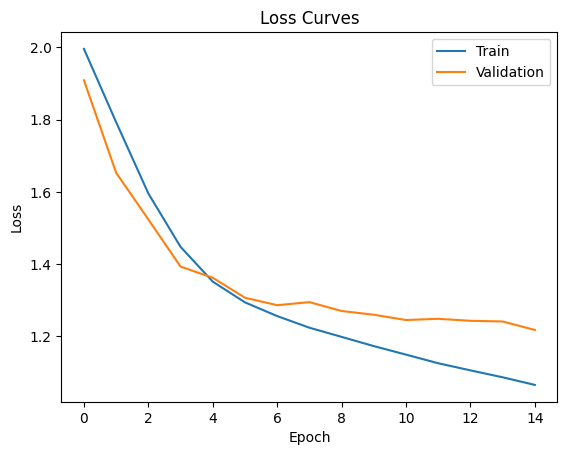
\includegraphics[width=0.8\textwidth]{figures/01_loss_curves.png}
    \caption{Curvas de pérdida y precisión del primer modelo con 100k de datos de entrenamiento.}
    \label{fig:loss_curves_100k}
\end{figure}
  
\begin{figure}[H]
    \centering
    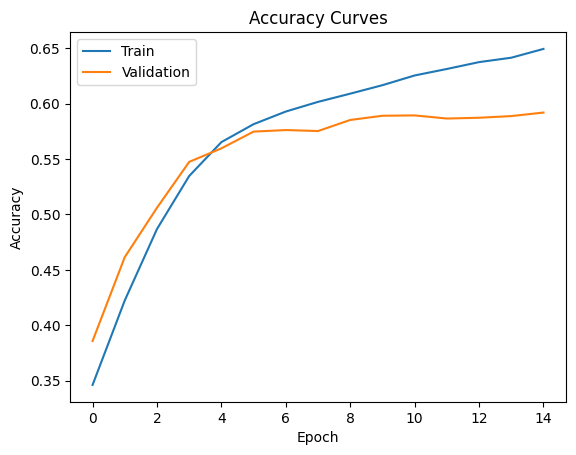
\includegraphics[width=0.8\textwidth]{figures/01_accuracy_curves.png}
    \caption{Curvas de pérdida y precisión del primer modelo con 100k de datos de entrenamiento.}
    \label{fig:accuracy_curves_100k}
\end{figure}

\begin{figure}[H]
    \centering
    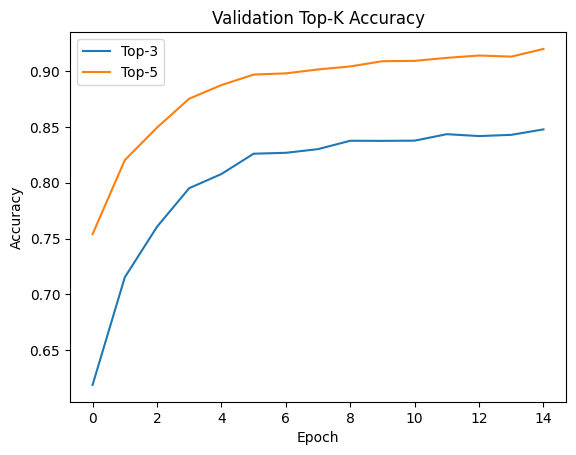
\includegraphics[width=0.8\textwidth]{figures/01_top_k_accuracy.png}
    \caption{Curvas de precisión top-k del primer modelo con 100k de datos de entrenamiento.}
    \label{fig:top_k_accuracy_100k}
\end{figure}
    
Con estos resultados obtuvimos un serie de observaciones importantes: la primera es que el modelo no llegó a la saturación de la precisión, lo que nos indica que el modelo no está sobreajustando los datos de entrenamiento y que podría mejorar con más datos de entrenamiento. La segunda observación es que apesar de que la precisión top-1 del modelo es de 0.65 para los datos de entrenamiento y 0.591 para los datos de valisación, la precisión top-3 es de 0.84 y la top-5 es de 0.91, lo que indica que el modelo es capaz de aprender a predecir los descartes de Mahjong a partir del diseño y la arquitectura que tenemos, y que con más datos de entrenamiento podría mejorar su precisión top-1.

A seguir podemos ver el gráfico de distribución de confianza del modelo, que nos permite ver la distribución de la probabilidad de los descartes predichos por el modelo.

\begin{figure}[H]
    \centering
    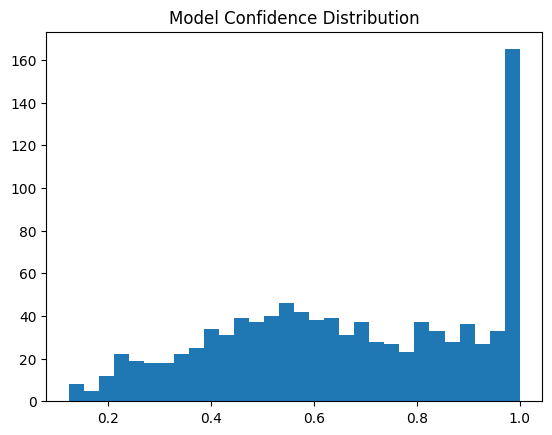
\includegraphics[width=0.8\textwidth]{figures/01_model_confidence.png}
    \caption{Distribución de confianza del primer modelo con 100k de datos de entrenamiento.}
    \label{fig:confidence_distribution_100k}
\end{figure}

Con este gráfico podemos ver que el modelo tiene un pico en la probabilidad de 1.0. Este pico indica una confianza del 100\% en muchas de las predicciones del modelo, no obstante, esta confianza puede ser explicada con los estados de juego en el que existe una única opción de descarte. Para arreglar esto, se realizó una limpieza de datos para eliminar los estados de juego en los que existe una única opción de descarte para el entrenamiento del próximo modelo, que será presentado a continuación.

\subsection{Segundo Modelo}

Este segundo modelo fue entrenado con 500k de datos de entrenamiento, 50k de validación y 50k de testeo. El modelo fue entrenado durante 15 épocas, con un batch size de 64 y un learning rate de 1e-4. A continuación se presentan las curvas de pérdida y precisión del modelo durante el entrenamiento de las épocas 9 a 15. El dataset de entrenamiento también fue limpiado para eliminar los estados de juego en los que existe una única opción de descarte.

\begin{figure}[H]
    \centering
    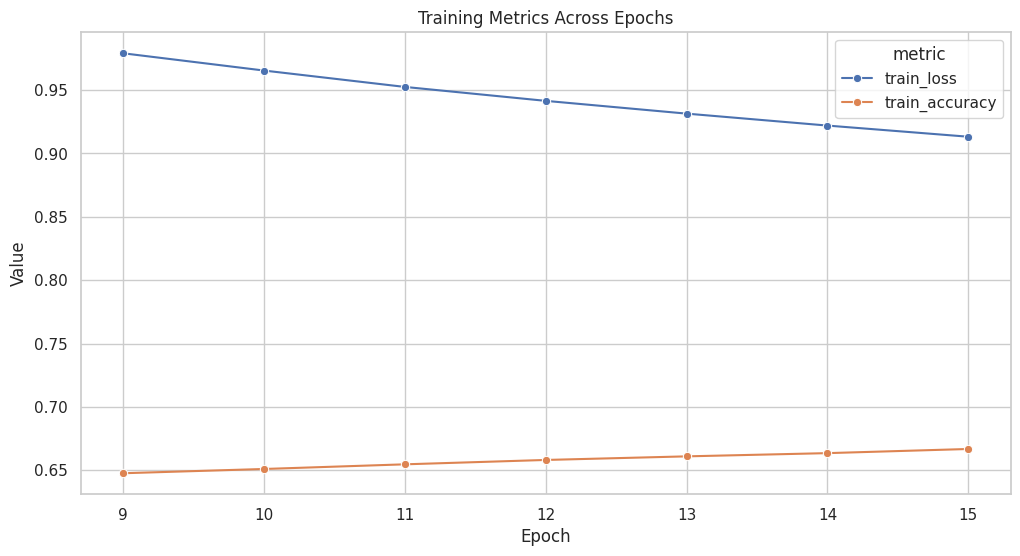
\includegraphics[width=0.8\textwidth]{figures/02_training_metrics.png}
    \caption{Curvas de pérdida y precisión del segundo modelo con 500k de datos de entrenamiento.}
    \label{fig:loss_curves_500k}
\end{figure}
    
Y en esta figura podemos ver el gráfico de distribución de confianza del modelo ajustado sin los estados de juego en los que existe una única opción de descarte.

\begin{figure}[H]
    \centering
    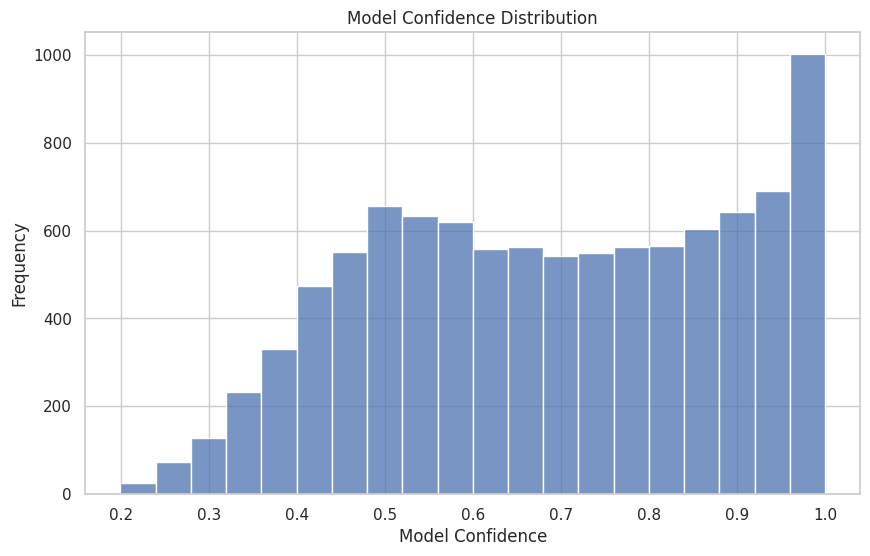
\includegraphics[width=0.8\textwidth]{figures/02_model_confidence.png}
    \caption{Distribución de confianza del segundo modelo con 500k de datos de entrenamiento.}
    \label{fig:confidence_distribution_500k}
\end{figure}

Podemos ver que pese a la disminución de la confianza del modelo, el modelo sigue teniendo un pico en la probabilidad de 1.0, lo que indica que el modelo sigue teniendo una confianza del 100\% en muchas de sus predicciones. Además de eso, podemos ver que la tiene un segundo pico en el 0.5 donde se mantiene estable hasta el 0.9. Estos resultados indican una buena confianza del modelo en sus predicciones, principalmente si consideramos que en su mayoria de los estados de juego existen 13 opciones de descarte posibles en media.

\subsection{Validación Estratégica}

La validación estratégica es un proceso que nos permite evaluar la capacidad del modelo para predecir descartes de Mahjong en función de la estrategia de juego. Para ello, se utilizaron métricas basadas en el Shanten y el Ukeire, que nos permiten clasificar los errores del modelo en diferentes categorías semánticas.

Las categorias creadas son las siguientes:

\begin{itemize}
    \item Exact match: el descarte predicho por el modelo coincide exactamente con el descarte real del jugador.
    \item Equivalent: el descarte predicho por el modelo resulta en el mismo Shanten y Ukeire que el descarte real del jugador.
    \item Better shanten: el descarte predicho por el modelo resulta en un Shanten menor que el descarte real del jugador.
    \item Better ukeire: el descarte predicho por el modelo resulta en un Ukeire mayor que el descarte real del jugador.
    \item Near equivalent: el descarte predicho por el modelo resulta en un Shanten y Ukeire que difieren en máximo dos unidades del descarte real del jugador.
    \item Shanten loss: el descarte predicho por el modelo resulta en un Shanten mayor que el descarte real del jugador.
    \item Ukeire loss: el descarte predicho por el modelo resulta en un Ukeire menor.
\end{itemize}

\subsubsection{Validación Estratégica del Primer Modelo}


A partir de 10k de datos de validación, de los cuales todos tienen por lo menos más de una opción de acción válida, se realizó la categorización de cada decisión tomada por la máquina utilizando las categorías mencionadas anteriormente.

En este primer gráfico podemos observar que muchas decisiones buenas, como \textit{better\_shanten} o \textit{better\_ukeire} no fueron llevadas en consideración al \textit{accuracy} del modelo:

\begin{figure}[H]
    \centering
    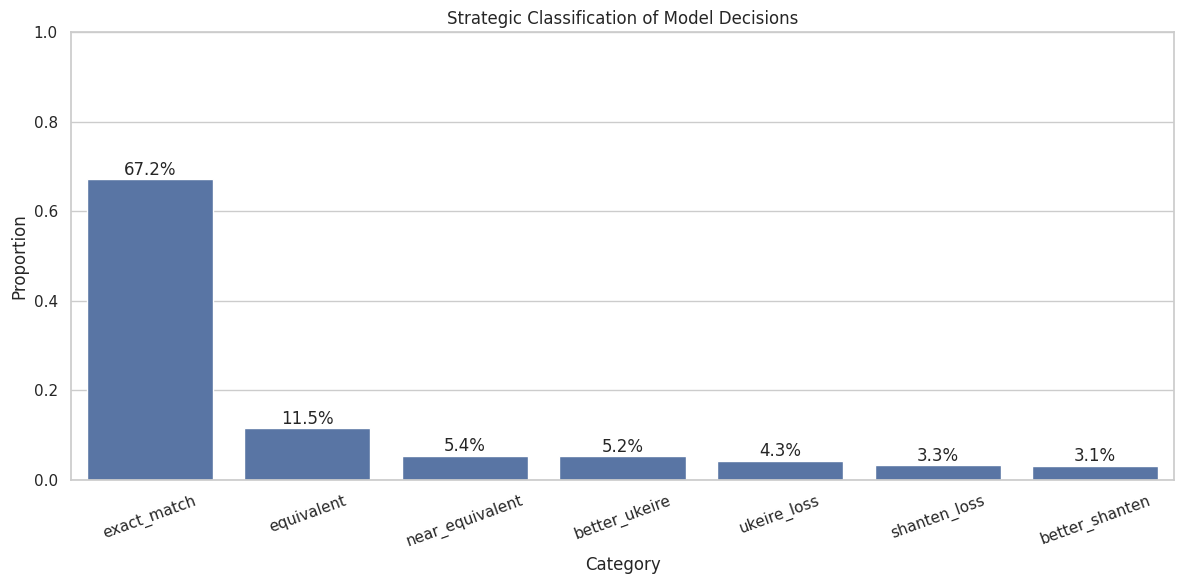
\includegraphics[width=0.8\textwidth]{figures/01_classificacion_estrategica.png}
    \caption{Porcentaje de Cada Categoría Estratégica en el Primer Modelo}
    \label{fig:strategic_class_100k}
\end{figure}

A partir de esto, podemos sacar un valor de \textit{strategic accuracy} mucho mejor que el \textit{accuracy} original, sumando las categorias de \textit{exact\_match, equivalent, better\_ukeire, better\_shanten} obtenemos que el modelo en realidad obtuvo una \textit{accuracy} de 92.4\%.

\begin{figure}[H]
    \centering
    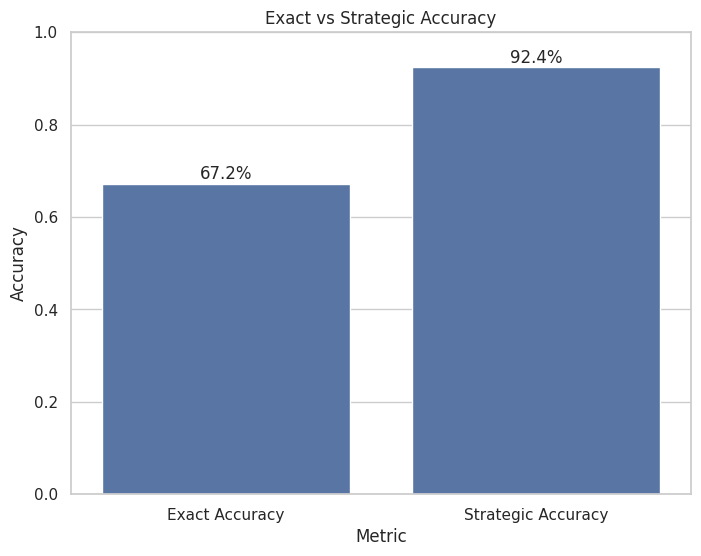
\includegraphics[width=0.8\textwidth]{figures/01_exactvstrategic.png}
    \caption{Comparación validación de accuracy exacta vs accuracy estratégica en el Primer Modelo}
    \label{fig:exact_vs_strat_100k}
\end{figure}

En esta figura también podemos ver la confianza dedl modelo sobre estos datos sin la interferencia de la confianza para datos de validación con una sola acción válida:

\begin{figure}[H]
    \centering
    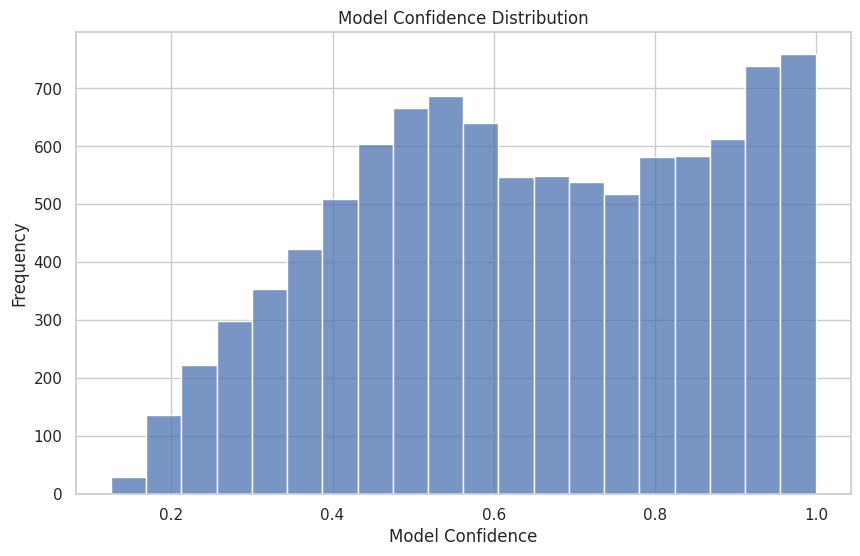
\includegraphics[width=0.8\textwidth]{figures/01_conf_dist_strat.png}
    \caption{Distribución de confianza del primer modelo con ajustado al dataset sin opciones unitárias}
    \label{fig:confidence_distribution_better_100k}
\end{figure}

Como podemos ver, la confianza del modelo está en rangos apropriados para el número de opciones que tiene normalmente (una media de 13 opciones).

Por último, podemos ver también la distribución de confianza del modelo por categoría estretégica, y se percibe que para los casos en que hubo errores graves la confianza del modelo es muy baja en comparación a la confianza en casos de exactitud del modelo, esto indica un buen aprendizaje del modelo.

\begin{figure}[H]
    \centering
    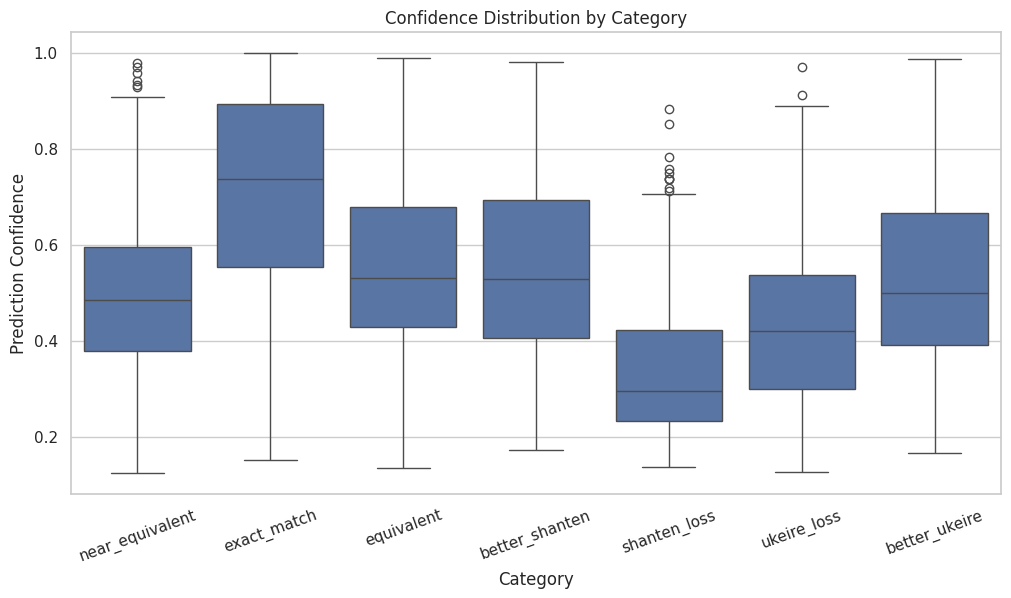
\includegraphics[width=0.8\textwidth]{figures/01_conf_dist_by_cat.png}
    \caption{Distribución de confianza del primer modelo por categoría de la validación estratégica}
    \label{fig:confidence_distribution_by_cat_100k}
\end{figure}

\subsubsection{Validación Estratégica del Segundo Modelo}
De manera análoga al análisis previo, se evaluaron 10k muestras de validación con múltiples opciones de acción válidas para el segundo modelo, aplicando la misma metodología de categorización estratégica.
Al inspeccionar la distribución de las decisiones, observamos cómo el aumento de datos impactan en la consideración de jugadas estratégicamente superiores como \textit{better\_shanten} o \textit{better\_ukeire}:
\begin{figure}[H]
\centering
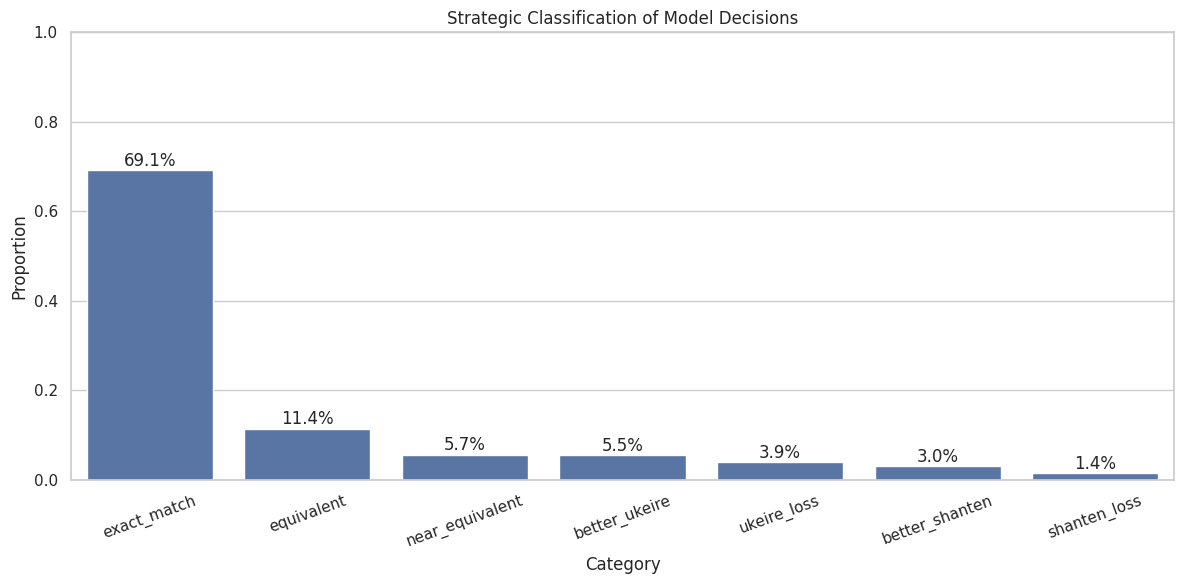
\includegraphics[width=0.8\textwidth]{figures/02_strategic_mistakes.png} 
\caption{Porcentaje de Cada Categoría Estratégica en el Segundo Modelo}
\label{fig:strategic_class_model2}
\end{figure}

Calculando nuevamente el \textit{strategic accuracy} acumulando las categorías de \textit{exact\_match, equivalent, better\_ukeire} y \textit{better\_shanten}, obtenemos un valor ajustado de \textbf{94.6\%}. Esto representa una mejora significativa respecto al accuracy crudo, demostrando que el modelo captura mejor la esencia estratégica del juego más allá de la coincidencia exacta:
\begin{figure}[H]
\centering
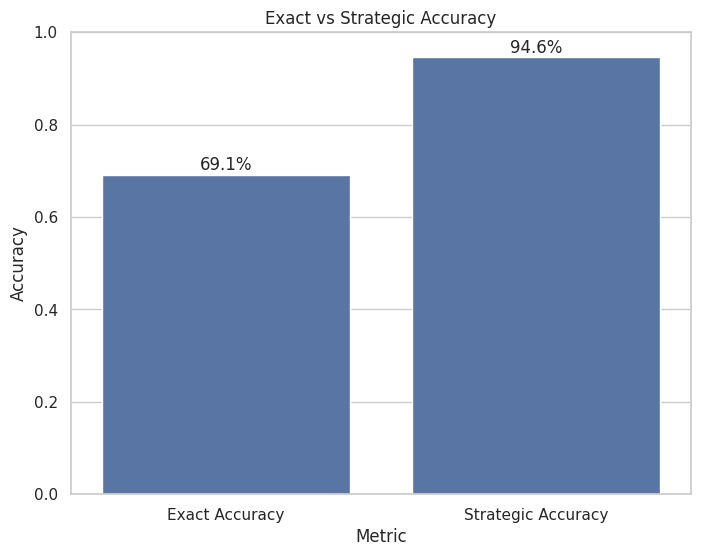
\includegraphics[width=0.8\textwidth]{figures/02_exatvstrategic.png} 
\caption{Comparación validación de accuracy exacta vs accuracy estratégica en el Segundo Modelo}
\label{fig:exact_vs_strat_model2}
\end{figure}

Respecto a la confianza del modelo, la distribución reflejada es bastante similar a la del primer modelo, pero aumenta consideramblemente la confianza en 100\%:
\begin{figure}[H]
\centering
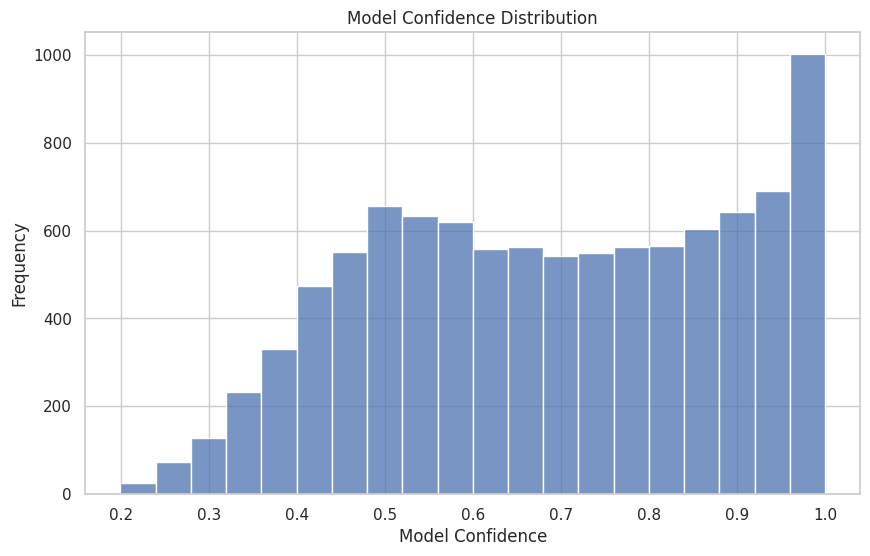
\includegraphics[width=0.8\textwidth]{figures/02_confidence_dist.png} 
\caption{Distribución de confianza del segundo modelo}
\label{fig:confidence_distribution_better_model2}
\end{figure}

Finalmente, podemos ver la descomposición de la confianza por categoría estratégica en este segundo modelo, donde más adelante se realizará una comparación entre los dos modelos:
\begin{figure}[H]
\centering
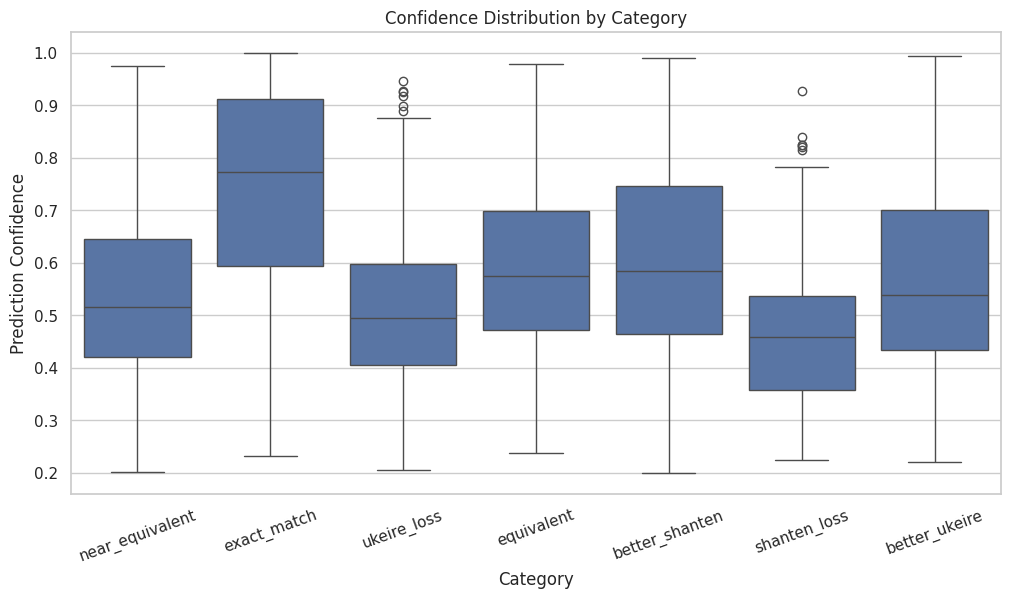
\includegraphics[width=0.8\textwidth]{figures/02_confidence_by_category.png}
\caption{Distribución de confianza del segundo modelo por categoría de la validación estratégica}
\label{fig:confidence_distribution_by_cat_model2}
\end{figure}

\subsubsection{Análisis Comparativo: Impacto del Volumen de Datos}
Para evaluar el impacto directo de la cantidad de datos en el rendimiento estratégico y exacto, se realizó una comparación entre el modelo entrenado con 100k muestras y aquel entrenado con 500k muestras.

En primer lugar, observamos que el aumento del conjunto de entrenamiento generó una mejora significativa en la \textit{exact action accuracy}. El modelo con 500k datos alcanzó un valor de $0.691$, superando al modelo con 100k, cuyo rendimiento se situó en $0.671$. Esta tendencia positiva también se reflejó en la métrica ajustada: el \textit{strategic accuracy} aumentó del $92.4\%$ al $94.6\%$, lo que indica una mayor capacidad del modelo para identificar acciones equivalentes o superiores desde una perspectiva estratégica general:
\begin{figure}[H]
\centering
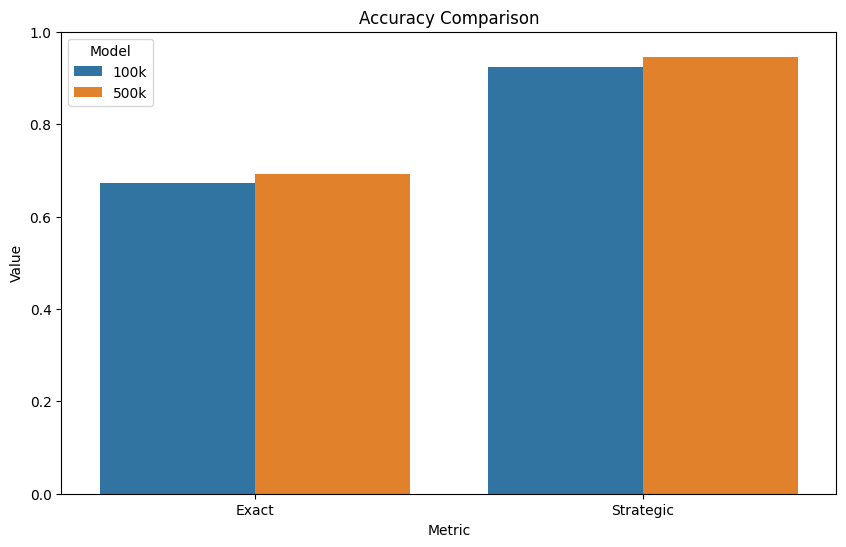
\includegraphics[width=0.8\textwidth]{figures/comparativa_exact_vs_strat.png} 
\caption{Comparación de Accuracy Exacta y Estratégica entre modelos con 100k y 500k de datos}
\label{fig:comp_exact_strat_acc}
\end{figure}

Al analizar la distribución específica por categorías estratégicas, resulta evidente un cambio cualitativo crucial en la toma de decisiones. El modelo entrenado con el conjunto más amplio redujo drásticamente la frecuencia de decisiones que degradan el estado del juego (\textit{shanten-degrading decisions}), pasando de un $3.4\%$ a solo un $1.8\%$. Esta reducción sugiere que el modelo no solo está memorizando respuestas exactas, sino aprendiendo patrones estructurales más profundos que evitan errores estratégicos graves:
\begin{figure}[H]
\centering
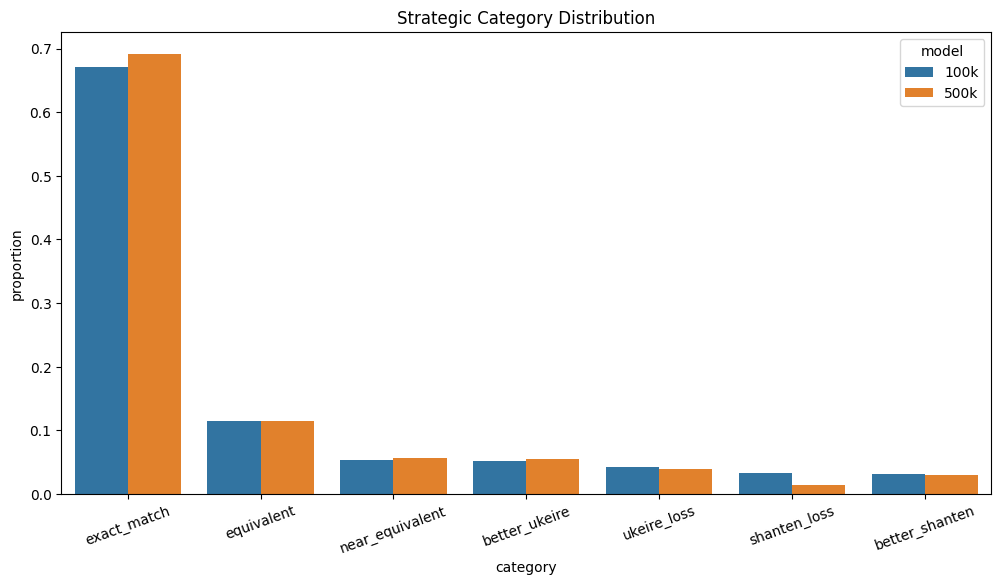
\includegraphics[width=0.8\textwidth]{figures/comparativa_categorias_estrategicas.png}
\caption{Comparación de la distribución de categorías estratégicas entre los dos modelos}
\label{fig:comp_strategic_categories}
\end{figure}

En conclusión, los resultados muestran que el incremento del conjunto de entrenamiento de 100k a 500k muestras produce una mejora consistente en prácticamente todas las métricas evaluadas. El segundo modelo aumenta tanto la \textit{exact accuracy} (67.16\% frente a 69.13\%) como la \textit{strategic accuracy} (92.43\% frente a 94.62\%), además de presentar una mayor confianza media en sus predicciones. Desde el punto de vista estratégico, también se observa una reducción importante de las decisiones que empeoran el Shanten y una mejora del \textit{Mean Ukeire Difference}, que pasa de un valor negativo a uno positivo. Aunque el porcentaje de decisiones clasificadas como \textit{Ukeire Loss} aumenta muy ligeramente (4.3\% frente a 4.4\%), este incremento es prácticamente despreciable y viene acompañado de un mayor número de decisiones \textit{Better Ukeire}, por lo que el balance global continúa siendo claramente favorable para el modelo entrenado con 500k muestras. Estos resultados indican que el aumento del volumen de datos no solo mejora la capacidad del modelo para reproducir decisiones expertas, sino también para realizar descartes estratégicamente más sólidos en una mayor variedad de situaciones de juego.

\section{Conclusiones y Líneas de Trabajo Futuro}

El objetivo principal de este trabajo ha sido estudiar la aplicación de arquitecturas Transformer al problema de la predicción de descartes en Riichi Mahjong mediante aprendizaje por imitación utilizando partidas reales de Tenhou. Para ello se diseñó una representación propia del estado de juego, un proceso de tokenización adaptado al dominio y un modelo basado en un Transformer Encoder capaz de aprender a seleccionar descartes a partir de ejemplos de jugadores expertos.

Los resultados obtenidos muestran que el modelo es capaz de aprender patrones relevantes para la selección de descartes a partir de los datos disponibles. Sobre un conjunto reservado de 52.563 estados, el modelo entrenado con 100.000 muestras alcanzó una precisión exacta del 55,81\% y una precisión estratégica del 88,97\%. El modelo entrenado con 500.000 muestras mejoró estos resultados hasta el 65,64\% y el 94,01\%, respectivamente. También aumentó la precisión top-3 del 83,37\% al 92,47\% y redujo la pérdida de 1,3533 a 0,9440.

Desde el punto de vista estratégico, el incremento del conjunto de entrenamiento redujo las decisiones que empeoran el Shanten del 5,03\% al 1,59\% y las decisiones que reducen significativamente el Ukeire del 6,00\% al 4,39\%. Estos resultados, obtenidos sobre estados no utilizados durante el entrenamiento, proporcionan una evidencia más sólida de la mejora introducida por el mayor volumen de datos. No obstante, debido a la ausencia de identificadores de partida, la separación se realizó por posición en la base de datos y no pudo garantizarse la independencia entre partidas.

No obstante, la principal aportación de este trabajo no reside únicamente en el desarrollo del modelo, sino en la metodología propuesta para su evaluación. Tradicionalmente, los modelos de aprendizaje por imitación suelen evaluarse mediante métricas de clasificación, como la exactitud (\textit{accuracy}), que consideran correcta únicamente la reproducción exacta de la acción realizada por el jugador experto. En un juego como el Riichi Mahjong, donde una misma situación puede admitir múltiples decisiones estratégicamente equivalentes, este criterio resulta insuficiente y puede conducir a conclusiones erróneas sobre la calidad real del modelo.

Con el objetivo de superar esta limitación, en este trabajo se propuso una validación estratégica basada en conceptos propios del Mahjong, como el Shanten y el Ukeire. Esta metodología permite distinguir entre errores realmente perjudiciales y decisiones alternativas que mantienen o incluso mejoran la calidad estratégica de la jugada. Gracias a este enfoque fue posible observar que una parte importante de las predicciones consideradas incorrectas por las métricas tradicionales corresponden, en realidad, a decisiones estratégicamente válidas o incluso superiores a las realizadas por el jugador experto.

Sin embargo, estas métricas no deben interpretarse como una medida absoluta de la inteligencia del modelo. Una precisión estratégica elevada no implica necesariamente que el sistema haya comprendido todos los aspectos del juego, sino únicamente aquellos representados por las heurísticas utilizadas durante la evaluación. En consecuencia, estas métricas deben entenderse como una herramienta de análisis que permite describir con mayor precisión el comportamiento del modelo, y no como una medida definitiva de su nivel de juego.

\section{Líneas de Trabajo Futuro}

Aunque los resultados obtenidos son prometedores, existen numerosas líneas de trabajo que permitirían ampliar y mejorar tanto el modelo desarrollado como la metodología de evaluación propuesta.

En primer lugar, una posible línea de investigación consiste en ampliar las métricas estratégicas utilizadas durante la evaluación. En este trabajo únicamente se consideraron el Shanten y el Ukeire como indicadores de calidad estratégica. Sin embargo, el Riichi Mahjong incorpora numerosas heurísticas adicionales relacionadas con el juego ofensivo y defensivo, como el Suji, Ura-Suji, Kabe, Genbutsu o el análisis del peligro de descarte frente a jugadores en Riichi. La incorporación de este tipo de criterios permitiría construir una evaluación mucho más completa del comportamiento estratégico del modelo.

De forma similar, la propia clasificación estratégica podría extenderse para analizar otros aspectos de la toma de decisiones, permitiendo estudiar no solamente si un descarte mejora la eficiencia de la mano, sino también si representa una decisión defensivamente adecuada o consistente con estrategias de mayor nivel empleadas por jugadores expertos.

Desde el punto de vista del modelo, otra línea de trabajo consiste en explorar arquitecturas más avanzadas. Aunque en este proyecto se ha empleado un Transformer Encoder relativamente sencillo para facilitar el análisis del comportamiento del sistema, existen variantes modernas como Decision Transformer o arquitecturas específicas para aprendizaje secuencial que podrían aprovechar mejor la naturaleza temporal de las partidas de Mahjong.

Asimismo, este trabajo se ha centrado exclusivamente en la decisión de descarte, que constituye la acción más frecuente durante una partida. Como continuación natural del proyecto, sería interesante ampliar el espacio de acciones para incluir decisiones como Chi, Pon, Kan, Riichi o incluso Tsumo y Ron. Esto permitiría construir un agente capaz de participar de manera completa en una partida real de Riichi Mahjong.

Finalmente, otra línea especialmente interesante consiste en utilizar el modelo obtenido mediante aprendizaje por imitación como punto de partida para un proceso posterior de aprendizaje por refuerzo. En este contexto, las métricas estratégicas desarrolladas en este trabajo podrían resultar útiles para el diseño de funciones de recompensa más informativas que la simple victoria o derrota al final de la partida. Incorporar información relacionada con el Shanten, el Ukeire o futuras heurísticas estratégicas permitiría proporcionar una señal de aprendizaje más densa durante el entrenamiento, facilitando potencialmente la convergencia del agente y favoreciendo la adquisición de comportamientos estratégicamente sólidos.


\clearpage
\section{Glosario}

Este glosario recoge los términos japoneses e ingleses empleados con mayor frecuencia. En los términos japoneses se incluye la grafía habitual en japonés y su romanización.

\subsection{Términos de Riichi Mahjong}

\begin{description}[style=nextline,leftmargin=4.2cm]
    \item[Riichi Mahjong --- {\japanesefont リーチ麻雀} (rīchi mājan)] Variante japonesa del Mahjong empleada en este trabajo.
    \item[Riichi --- {\japanesefont 立直／リーチ} (rīchi)] Declaración realizada cuando una mano cerrada queda en Tenpai, acompañada del depósito de 1.000 puntos.
    \item[Shanten --- {\japanesefont 向聴数／シャンテン数} (shanten-sū)] Distancia estructural de una mano respecto de Tenpai. Un valor menor indica que la mano está más cerca de completarse.
    \item[Tenpai --- {\japanesefont 聴牌／テンパイ} (tenpai)] Estado en el que falta una sola ficha válida para completar la mano.
    \item[Ukeire --- {\japanesefont 受け入れ／ウケイレ} (ukeire)] Número de copias todavía disponibles de las fichas que mejoran el Shanten de la mano.
    \item[Dora --- {\japanesefont ドラ} (dora)] Ficha que aporta valor adicional a una mano ganadora, determinada a partir de un indicador.
    \item[Aka Dora --- {\japanesefont 赤ドラ} (aka dora)] Cinco rojo que cuenta como Dora.
    \item[Tsumo --- {\japanesefont 自摸／ツモ} (tsumo)] Robo de una ficha; también, victoria obtenida con una ficha robada por el propio jugador.
    \item[Tsumogiri --- {\japanesefont ツモ切り} (tsumogiri)] Descarte inmediato de la misma ficha que se acaba de robar.
    \item[Ron --- {\japanesefont ロン} (ron)] Victoria conseguida utilizando la ficha descartada por otro jugador.
    \item[Chi --- {\japanesefont チー} (chī)] Llamada que forma una secuencia con el descarte del jugador situado a la izquierda.
    \item[Pon --- {\japanesefont ポン} (pon)] Llamada que forma un trío con una ficha descartada por otro jugador.
    \item[Kan --- {\japanesefont 槓／カン} (kan)] Grupo de cuatro fichas idénticas. Puede ser cerrado, abierto o ampliado.
    \item[Ankan --- {\japanesefont 暗槓} (ankan)] Kan cerrado formado con cuatro fichas propias.
    \item[Daiminkan --- {\japanesefont 大明槓} (daiminkan)] Kan abierto completado mediante el descarte de otro jugador.
    \item[Shouminkan o Kakan --- {\japanesefont 小明槓／加槓} (shōminkan/kakan)] Ampliación de un Pon abierto al añadir la cuarta ficha.
    \item[Mentsu --- {\japanesefont 面子} (mentsu)] Grupo que forma parte de una mano: secuencia, trío o Kan.
    \item[Fūro --- {\japanesefont 副露} (fūro)] Grupo expuesto mediante una llamada a una ficha de otro jugador.
    \item[Yaku --- {\japanesefont 役} (yaku)] Patrón o condición que concede valor y permite que una mano pueda ganar.
    \item[Furiten --- {\japanesefont 振聴／フリテン} (furiten)] Situación que impide ganar por Ron sobre las esperas afectadas, aunque todavía puede ser posible ganar por Tsumo.
    \item[Honba --- {\japanesefont 本場} (honba)] Contador de rondas consecutivas que incrementa los pagos de la mano.
    \item[Kyūshukyūhai --- {\japanesefont 九種九牌} (kyūshukyūhai)] Opción de abortar la mano inicial cuando se cumplen las condiciones de fichas terminales y de honor distintas.
    \item[Chankan --- {\japanesefont 槍槓} (chankan)] Victoria al reclamar la ficha con la que otro jugador intenta ampliar un Kan.
    \item[Suji --- {\japanesefont 筋} (suji)] Heurística defensiva basada en las relaciones entre esperas de secuencia.
    \item[Kabe --- {\japanesefont 壁} (kabe)] Heurística defensiva que aprovecha las fichas visibles para descartar ciertas esperas posibles.
    \item[Genbutsu --- {\japanesefont 現物} (genbutsu)] Ficha ya descartada por un jugador en Riichi y, por ello, segura contra su Ron mientras se mantenga esa situación.
    \item[Ura-suji --- {\japanesefont 裏筋} (ura-suji)] Patrón defensivo relacionado con posibles esperas situadas alrededor de un descarte.
\end{description}

\subsection{Términos técnicos en inglés}

\begin{description}[style=nextline,leftmargin=4.2cm]
    \item[Accuracy] Exactitud: proporción de predicciones que cumplen el criterio considerado correcto.
    \item[Batch] Lote de muestras procesadas conjuntamente durante el entrenamiento o la evaluación.
    \item[Checkpoint] Fichero que conserva los parámetros de un modelo en un momento determinado.
    \item[Dataset] Conjunto de datos utilizado para el entrenamiento o la evaluación.
    \item[Dropout] Técnica de regularización que desactiva aleatoriamente parte de las activaciones durante el entrenamiento.
    \item[Embedding] Representación vectorial aprendida de un identificador discreto.
    \item[Encoder] Componente que transforma una secuencia de entrada en representaciones contextuales.
    \item[Feed-forward] Red neuronal aplicada de forma independiente a cada posición dentro de una capa Transformer.
    \item[Holdout] Conjunto reservado que no se utiliza para entrenar el modelo y se emplea en la evaluación final.
    \item[Logit] Puntuación no normalizada producida por el modelo antes de aplicar una distribución de probabilidad.
    \item[Mask] Máscara que indica qué posiciones deben atenderse o ignorarse durante el procesamiento.
    \item[Policy head] Capa de salida que asigna una puntuación a cada acción candidata.
    \item[Self-attention] Mecanismo que relaciona cada elemento de una secuencia con los demás elementos de esa misma secuencia.
    \item[Softmax] Función que transforma un conjunto de logits en una distribución de probabilidad.
    \item[Token] Unidad discreta utilizada para representar una parte de la entrada del modelo.
    \item[Top-k accuracy] Proporción de ejemplos en los que la acción observada aparece entre las $k$ predicciones con mayor puntuación.
    \item[Transformer] Arquitectura neuronal basada principalmente en mecanismos de atención.
\end{description}


\clearpage

\printbibliography

\end{document}